\documentclass[compress,usepdftitle=false,xcolor=pdftex,svgnames,table,aspectratio=169]{beamer}

%\setbeameroption{show notes on second screen=right}
% Notes
% \usepackage{pgfpages}
% \setbeameroption{show notes on second screen=right}

%\definecolor{bluegreen}{RGB}{3, 166, 155}
%\definecolor{pitchblack}{RGB}{0, 0, 0}
%\definecolor{lightbeige}{RGB}{255, 251, 241}
%\definecolor{mediumgray}{RGB}{183, 183, 183}

%\setbeamercolor{background canvas}{bg=pitchblack}
\setbeamercolor{normal text}{fg=black}
\setbeamercolor{frametitle}{bg=LightGrey, fg=black}
\setbeamercolor{title}{fg=black, bg=white}
\definecolor{blockcolor}{RGB}{250, 250, 200}
\setbeamercolor{block}{fg=black, bg=blockcolor}
\setbeamercolor{sticky}{fg=black, bg=blockcolor}
%\usetheme{plain}
%\useoutertheme[subsection=false]{miniframes}
\usefonttheme{professionalfonts}
%%\setbeamercolor{section in head/foot}{fg=white, bg=black}
%% \setbeamercolor{mini frame}{fg=white, bg=black}
\usebeamercolor[fg]{title in head/foot}
\usefonttheme[onlylarge]{structurebold}
\setbeamerfont*{frametitle}{size=\normalsize,series=\bfseries}
\setbeamertemplate{navigation symbols}{}
%%\setbeamertemplate{headline}[miniframes theme]{}
%\setbeamertemplate{footline}[default]
%\defbeamertemplate{footline}{centered page number}
%{%
%  \hspace*{\fill}%
%  \usebeamercolor[fg]{page number in head/foot}%
%  \usebeamerfont{page number in head/foot}%
%  \insertpagenumber\,/\,\insertpresentationendpage%
%  \hspace*{\fill}\vskip2pt%
%}
%\setbeamertemplate{footline}[centered page number]
\setbeamertemplate{footline}[frame number]
\setbeamertemplate{bibliography entry title}{}
\setbeamertemplate{bibliography entry location}{}
\setbeamertemplate{bibliography entry note}{}

%\setbeamercolor{background canvas}{bg=LightGrey}

\makeatletter
\setbeamertemplate{title page}[default][left,colsep=-4bp,rounded=true]
\makeatother
\setbeamerfont{frametitle}{size=\LARGE}
\setbeamerfont{title}{size=\Huge}
\setbeamerfont{author}{size=\Large}
\setbeamerfont{institute}{size=\large}

\setbeamercolor*{block title alerted}{fg=black, bg=red!40}
\setbeamercolor*{block body alerted}{fg=black, bg=red!25}
\setbeamerfont{alerted text}{series=\bfseries}
\setbeamercolor{alerted text}{fg=blue, bg=white}

\setbeamercolor*{block title example}{fg=blue!50, bg=blue!10}
\setbeamercolor*{block body example}{fg= blue, bg=blue!5}

\newcommand\mailto[1]{\href{mailto: #1}{#1}}

\newcommand\redbf[1]{{\color{red}\textbf{#1}}}

\setbeamertemplate{itemize item}{\scriptsize\raise1.25pt\hbox{\textbullet}}
\setbeamertemplate{itemize subitem}{\tiny\raise1.5pt\hbox{\textbf{--}}}
\setbeamertemplate{itemize subsubitem}{\tiny\raise1.5pt\hbox{\textbf{--}}}
\setbeamertemplate{enumerate item}{\insertenumlabel.}
\setbeamertemplate{enumerate subitem}{\insertenumlabel.\insertsubenumlabel}
\setbeamertemplate{enumerate subsubitem}{\insertenumlabel.\insertsubenumlabel.\insertsubsubenumlabel}
\setbeamertemplate{enumerate mini template}{\insertenumlabel}
\setbeamercolor{itemize item}{fg=gray}
\setbeamercolor{itemize subitem}{fg=gray}
\setbeamercolor{itemize subsubitem}{fg=gray}

\newcommand{\highl}[1]{%
  \colorbox{yellow!30}{$\displaystyle#1$}}

\usepackage{tikz}
  \usetikzlibrary{calc,decorations.pathreplacing,
    decorations.pathmorphing,
    decorations.markings,
    shapes, fit,
    arrows.meta, tikzmark
    }
  \usetikzlibrary{cd}
  \usetikzlibrary{positioning}
  \usetikzlibrary{arrows}

\tikzset{
    arrow at end/.style={
        decorate,decoration={
            markings,
            mark=at position .999 with{
                \arrow{#1};
            }
        }
    }
}

\usepackage[skins]{tcolorbox}

\newtcolorbox{sticky}[1][]
{%
  enhanced,
  center upper,
  fontupper=\strut,
  drop fuzzy shadow southeast,
  boxrule=0pt,
  sharp corners,
  colframe=yellow!80!black,
  colback=yellow!10,
  #1
}

\newtcolorbox{infobox}[1][]
{%
  enhanced,
  %center upper,
  drop fuzzy shadow southeast,
  boxrule=0pt,
  sharp corners,
  colframe=red!10,
  colback=red!10,
  #1
}

\newtcolorbox{bluebox}[1][]
{%
  enhanced,
  %center upper,
  drop fuzzy shadow southeast,
  boxrule=0pt,
  sharp corners,
  colframe=blue!10,
  colback=blue!10,
  #1
}

\newtcolorbox{greenbox}[1][]
{%
  enhanced,
  %center upper,
  drop fuzzy shadow southeast,
  boxrule=0pt,
  sharp corners,
  colframe=green!10,
  colback=green!10,
  #1
}
\usepackage{microtype}
\newsavebox\CBox
\newcommand<>*\textBF[1]{\sbox\CBox{#1}\resizebox{\wd\CBox}{\ht\CBox}{\textbf#2{#1}}}
\usepackage{tabularx}
\usepackage[framemethod=TikZ]{mdframed}

\usepackage{soul}

\newmdenv[
  topline=false,
  bottomline=false,
  rightline=false,
  skipabove=\topsep,
  skipbelow=\topsep,
  linewidth=1pt,
  linecolor=cyan
]{titlerule}

\setbeamertemplate{frametitle}{%
  \begin{titlerule}
    \usebeamerfont{frametitle}\insertframetitle\strut%
    \vskip-.2\baselineskip%
    % \leaders\vrule width \paperwidth\vskip0.4pt%
    \vskip0pt%
    \nointerlineskip
  \end{titlerule}
}


%% Terms
\newcommand\aWrap[1]{#1}
\newcommand\aConst[1]{\kw{const} \; #1}
\newcommand\aId{\kw{id}}
\newcommand\aComp{\mathbin{\circ}}
\newcommand\aProj[1]{\pi_{#1}}
\newcommand\aSplit{\mathbin{\vartriangle}}
\newcommand\aInj[1]{\kw{inj}_{#1}}
\newcommand\aCase{\mathbin{\triangledown}}
\newcommand\aIn{\kw{in}}
\newcommand\aOut{\kw{out}}
\newcommand\aRec{\kw{rec}}

\newcommand\mSend{\mathtt{send}}
\newcommand\mRecv{\mathtt{recv}}
\newcommand\mRet{\mathtt{return}}
\newcommand\mBind{\mathbin{{\tt >}\!\!{\tt >}\!{\tt =}}}
\newcommand\mComp{\mathbin{{\tt >}\!\!{\tt =}\!\!{\tt >}}}
\newcommand\mPar{\mathbin{\wedge}}
\newcommand\mChoice{\mathtt{choice}}
\newcommand\mBranch{\mathtt{branch}}

\newcommand\WF{\mathsf{WF}}
\newcommand\pexp{\text{\color{blue}{\tt e}}}
\newcommand\Gen[1]{\left\llbracket #1 \right\rrbracket}
\newcommand\AT{\text{\tt @}}

\newcommand\lSend[1]{!\langle #1 \rangle}
\newcommand\lRecv[1]{?(#1)}


\definecolor{dgreen}{RGB}{0,160,0}

\renewcommand\UrlFont{\color{red}\rmfamily\itshape}

\newcommand\vc[1]{\mathsf{#1}}

\usepackage{bm}
  \newcommand\role[1]{\mathsf{\bm{#1}}}
  \newcommand\kw[1]{\mathtt{#1}}
  \newcommand\kww[1]{\bm{\mathsf{#1}}}
  \newcommand\size[1]{\mathsf{#1}}
  \newcommand\crecv{c_{\mathsf{i}}}
  \newcommand\cost{C}
  \newcommand\Time{\mathcal{T}}
  \newcommand\Queue{\mathcal{Q}}
  \newcommand\addcost{\hookrightarrow}
  \newcommand\hasCost{\diamond}
  \newcommand\csend{c_{\mathsf{o}}}
  \newcommand\gMsgt{\rightsquigarrow}
  \newcommand\gMsg{\to}
  \newcommand\gFix{\mu}
  \newcommand\gEnd{\kw{end}}
  \newcommand\act{\alpha}
  \newcommand\unroll{\mathsf{unfold}}
  \newcommand\tRun{{\diamond}}
  % \newcommand{\rulename}[1]{\lbrack \text{#1}\rbrack}
  \newcommand\tSend{\mathbin{!}}
  \newcommand\tRecv{\mathbin{?}}
  \newcommand\tSelect{\mathbin{\oplus}}
  \newcommand\tBranch{\mathbin{\&}}
  \newcommand\gEval{\tRun}
  \newcommand\gTy[1]{ : \{#1\}}

\usepackage{minted}

\titlegraphic{%
  \begin{picture}(382,0)
    {\put(220,-10){\includegraphics[width=4cm]{figures/UoK_Logo.jpg}}}
  \end{picture}
  }

\title{Mechanising Recursion Schemes with Magic-Free Coq Extraction}
\author{\small\textbf{David Castro-Perez}, Marco Paviotti, and Michael Vollmer}
\institute{\mailto{d.castro-perez@kent.ac.uk}}
\date
}

\newcommand{\embf}[1]{\textbf{\emph{#1}}}
\newcommand{\mhask}[1]{\text{\mintinline{Haskell}{#1}}}
\newmintinline[haskell]{haskell}{fontsize=\small}
\newmintinline[coq]{coq}{fontsize=\small}
\newmintinline[ocaml]{OCaml}{fontsize=\small}
\newminted{coq}{fontsize=\small}
\newminted{ocaml}{fontsize=\small}
\newminted{haskell}{fontsize=\small}

\newcommand\sbullet[1][.5]{\mathbin{\vcenter{\hbox{\scalebox{#1}{$\bullet$}}}}}

\usepackage{stmaryrd}
\usepackage{mathpartir}

\newcommand\blfootnote[1]{%
  \begingroup
  \renewcommand\thefootnote{}\footnote{#1}%
  \addtocounter{footnote}{-1}%
  \endgroup
}

\definecolor{golden}{rgb}{0.99, 0.76, 0.0}

\tikzstyle{label}=[%
  shading = axis,
  rectangle,
  rounded corners,
  left color=golden,
  right color=golden!40!white,
  shading angle=180,
  anchor=north]

\def\Put(#1,#2)#3{\leavevmode\makebox(0,0){\put(#1,#2){#3}}}

\newcommand<>\highlightbox[2]{%
  \alt#3{\makebox[\dimexpr\width-2\fboxsep]{\colorbox{#1}{#2}}}{#2}%
}

\newcommand{\mathcolorbox}[2]{\colorbox{#1}{$\displaystyle #2$}}

\usepackage{amsmath}
\usepackage{amssymb}
\usepackage{latexsym}
\usepackage{amstext}
\usepackage{xspace}
\usepackage[svgnames]{xcolor}
\usepackage{mathtools}
\usepackage{cleveref}

\usepackage{etoolbox}

%% macros for colours in the syntax

% \def\NOCOLOR{} % define to remove color from the syntax

\ifdefined\NOCOLOR%
  \newcommand{\withcolor}[2]{#2} % no color selected
\else
  % sets and restores the color
  \newcommand{\withcolor}[2]{\colorlet{currbkp}{.}\color{#1}{#2}\color{currbkp}}
\fi


% colours for syntactic categories

\definecolor{amethyst}{rgb}{0.6, 0.4, 0.8}

\newcommand{\colorch}{Green} % colour for channel vars
\newcommand{\colorex}{Blue} % colour for expresion vars % Tomato was too bright
\newcommand{\colorexpvar}{Red} % colour for expression variables
\newcommand{\colorpart}{Teal} % colour for participants
\newcommand{\colorlbl}{Indigo} % colour for labels

\newcommand{\colorproc}{Maroon} % colour for processes
\newcommand{\colorprocvar}{Red} % colour for process variable (recursion)

\newcommand{\colorexp}{Blue} % colour for expressions

\newcommand{\colortpexp}{Orchid} % colour for the types of expressions
\newcommand{\colorgt}{VioletRed} % colour ofr global types

\newcommand{\colorsess}{DarkOrchid} % colour for multiparty sessions
\newcommand{\colorlt}{NavyBlue} % colour for local types

% Judgments and general macros

\newcommand{\code}[1]{\texttt{#1}}
\newcommand{\enc}[1]{\llbracket #1 \rrbracket}
\newcommand{\proj}{\upharpoonright}
% \newcommand{\setof}[1]{\{{#1}\}}
\newcommand{\subj}[1]{\operatorname{subj}(#1)}
\newcommand{\parts}[1]{\operatorname{parts}(#1)}

\newcommand{\bigstepsto}[1]{\ensuremath{\mathrel{\Downarrow}{#1}}}
\newcommand{\stepsto}[1]{\xrightarrow{#1}}
\newcommand{\evalsto}{\mathrel{\longrightarrow^*}}
\newcommand{\sstepsto}{\mathrel{\longrightarrow}} % static evaluation (expressions without communications)
\newcommand{\oft}[0]{\ensuremath{\mathrel{:}}}
\renewcommand{\emptyset}{\varnothing}
\newcommand{\freen}[1]{\ensuremath{\operatorname{fn}(#1)}}
\newcommand{\subst}[2]{\ensuremath{[\dex{#1}\mathrel{:=}{#2}]}}

\newcommand{\ie}[0]{i.e.\xspace}
\newcommand{\eg}[0]{e.g.\xspace}
\newcommand{\cf}[0]{cf.\xspace}

% Syntactic categories

\newcommand{\globalt}[1]{\withcolor{\colorgt}{#1}} % colour for global types
\newcommand{\localt}[1]{\withcolor{\colorlt}{#1}} % colour for local types

\newcommand{\expt}[1]{\withcolor{\colortpexp}{#1}} % colour for types of expressions and comm. types

% \newcommand{\dlt}[1]{\withcolor{\colorlt}{#1}} % colour for local types

\newcommand{\dev}[1]{\withcolor{\colorexpvar}{#1}} % colour for process variables

\newcommand{\dlbl}[1]{\withcolor{\colorlbl}{#1}} % colour for labels

\newcommand{\dpart}[1]{\withcolor{\colorpart}{\sf #1}} % colour for participants

\newcommand{\expr}[1]{\withcolor{\colorex}{#1}} % colour for expressions
\newcommand{\proc}[1]{\withcolor{\colorproc}{#1}} % colour for processes
\newcommand{\sess}[1]{\withcolor{\colorproc}{#1}} % colour for sessions
\newcommand{\pvar}[1]{\withcolor{\colorprocvar}{#1}} % colour for  process variables

% Some roles and labels

\newcommand{\Rp}{\dpart{p}}
\newcommand{\Rq}{\dpart{q}}
\newcommand{\Rr}{\dpart{r}}
\newcommand{\Rs}{\dpart{s}}
\newcommand{\Rpi}{\dpart{p'}}
\newcommand{\Rqi}{\dpart{q'}}
\newcommand{\Rri}{\dpart{r'}}
\newcommand{\Rsi}{\dpart{s'}}

\newcommand{\Sm}{\sess{\mathcal{M}}}
\newcommand{\Smi}{\sess{\mathcal{M}'}}

\newcommand{\lbl}{\ensuremath\dlbl{\ell}}
\newcommand{\lbli}{\ensuremath\dlbl{\ell'}}

% Process syntax

\newcommand{\psend}[4]{\ensuremath{\proc{\dpart{#1} \mathrel{!} \dlbl{#2}\langle\expr{#3}\rangle.\proc{#4}}}}
\newcommand{\precv}[3]{\ensuremath{\proc{\displaystyle\sum_{#1\in#2}\,{#3}}}}
\newcommand{\precbr}[4]{\ensuremath{\proc{\dpart{#1}?\dlbl{#2}(\dev{#3}).\proc{#4}}}}
\newcommand{\pif}[3]{\ensuremath{\proc{\code{if}\,\expr{#1}\,\code{then}\,\proc{#2}\,\code{else}\,\proc{#3}}}}
\newcommand{\precur}[2]{\ensuremath{\proc{\code{rec}\,\pvar{#1}\,.\,\proc{#2}}}}
\newcommand{\pfinish}{\ensuremath{\proc{\code{done}}}}

\newcommand{\snil}{\ensuremath{\sess{\cdot}}}
\newcommand{\scons}[3]{\ensuremath{\sess{\dpart{#1}\triangleleft\proc{#2}\mathrel{::}\sess{#3}}}}

\newcommand{\supdate}[3]{\ensuremath{\sess{{#1}[\dpart{#2}\triangleleft\proc{#3}]}}}

\newcommand{\spart}[2]{\ensuremath{\sess{\dpart{#1}\triangleleft\proc{#2}}}}
% \newcommand{\spar}[2]{\ensuremath{\sess{#1 \parallel #2}}}

% Global types

\newcommand{\gmsg}[3]{\ensuremath{\globalt{\dpart{#1}\to\dpart{#2}:{#3}}}}
\newcommand{\gmsgbr}[3]{\ensuremath{\globalt{\{\dlbl{#1}(\expt{#2}).{\globalt{#3}\}}}}}
\newcommand{\grecur}[2]{\ensuremath{\globalt{\mu{\pvar{#1}.\globalt{#2}}}}}
\newcommand{\gfinish}{\ensuremath{\globalt{\varnothing}}}

% Local types

\newcommand{\lsend}[2]{\ensuremath{\localt{\dpart{#1} ! {#2}}}}
\newcommand{\lrecv}[2]{\ensuremath{\localt{\dpart{#1} ? {#2}}}}
\newcommand{\lmsgbr}[3]{\ensuremath{\localt{\{\dlbl{#1}(\expt{#2}).{\localt{#3}\}}}}}
\newcommand{\lrecur}[2]{\ensuremath{\localt{\mu{\pvar{#1}.\localt{#2}}}}}
\newcommand{\lfinish}{\ensuremath{\localt{\varnothing}}}

% expression sorts

\newcommand{\sbool}[0]{\ensuremath{\expt{\code{bool}}}}
\newcommand{\snat}[0]{\ensuremath{\expt{\code{nat}}}}

% Global type LTS

\newcommand{\annlbl}[3]{\ensuremath{\dlbl{\overset{\dlbl{#3}}{{\dpart{#1}\!\to\!\dpart{#2}}}}}}

\newcommand{\greduceX}[4]{\ensuremath{\globalt{#2}\mathrel{\backslash}_{\sf #1}\!\dlbl{#3}\ifblank{#4}{}{=\globalt{#4}}}}

\newcommand{\greducehd}[3]{\greduceX {H} {#1}{#2}{#3}}
\newcommand{\greducetl}[3]{\greduceX {T} {#1}{#2}{#3}}
\newcommand{\greduce}[3]{\greduceX {} {#1}{#2}{#3}}

\newcommand{\lmerge}{\ensuremath{\localt{\sqcap}}}

\newcommand{\loft}[3]{\ensuremath{\globalt{#1}\vdash\proc{#2}\oft{\localt{#3}}}}
\newcommand{\toft}[3]{\ensuremath{\globalt{#1}\vdash\expr{#2}\oft{\expt{#3}}}}

% Typing judgments

\newcommand{\gproj}[2]{\ensuremath{\globalt{#1}\proj\dpart{#2}}}

\newcommand{\poft}[4]{\ensuremath{\globalt{#1}\vdash\proc{#2}\oft\gproj{#3}{#4}}}
\newcommand{\soft}[3]{\ensuremath{\vdash\sess{#1}\oft\globalt{#2}\Rightarrow\dpart{#3}}}

% Other expressions

\newcommand{\bisim}{\ensuremath{\mathrel{\,\sim\,}}}

%% Local Variables:
%% mode: latex
%% TeX-master: "main"
%% End:


\begin{document}
\frame[plain]{\titlepage}
%!TEX root = ../slides.tex
%\begin{frame}
%  \vfill
%  \centering
%  %\begin{beamercolorbox}[sep=8pt,center,shadow=true,rounded=true]{block}
%  \begin{sticky}
%    \usebeamerfont{title}
%    {\normalfont\Large MultiParty Session Types} \par%
%  \end{sticky}
%  %\end{beamercolorbox}
%  \vfill
%\end{frame}
%
\begin{frame}
  \vfill
  \centering
  %\begin{beamercolorbox}[sep=8pt,center,shadow=true,rounded=true]{block}
  \begin{sticky}
    \usebeamerfont{title}
    {\normalfont \textbf{Background and Motivation}}

    {\normalfont\Large A Crash Course on Classic Multiparty Session Types}
    \par%
  \end{sticky}
  %\end{beamercolorbox}
  \vfill
\end{frame}

\begin{frame}[fragile]{What is wrong with this code?}
  \scriptsize
  \begin{lstlisting}[language=Golang,
  belowskip=-0.6\baselineskip, aboveskip=-0.1\baselineskip]
func Worker(n int, resp chan int, err chan error) { ... }
func Master(reqCh chan int, respCh chan []int, cErrCh chan error) {
  for {
    ubound := <-reqCh
    workerChs := make([]chan int, ubound)
    errCh := make(chan error)
    for i := 0; i < ubound; i++ {
      workerChs[i] = make(chan int)
      go Worker(i+1, workerChs[i], errCh)
    }
    var res []int
    for i := 0; i < ubound; i++ {
      select {
      case sqI := <-workerChs[i]:
        res = append(res, sqI)
      case err := <-errCh:
        cErrCh <- err
        return
      }}
    respCh <- res}}
\end{lstlisting}
  \Put(40,290){%
    \begin{onlyenv}<2>
    \begin{minipage}{.86\columnwidth}
    \begin{infobox}
      \Large
      \textbf{DEADLOCK!}\vspace{.2cm}\\
      \textbf{ORPHAN MESSAGES!}\vspace{.2cm}\\
      \textbf{NO RESOURCE CLEANUP!}\vspace{.2cm}\\
      \textbf{...}
    \end{infobox}
    \end{minipage}
    \end{onlyenv}
    \begin{onlyenv}<3>
    \begin{minipage}{.86\columnwidth}
    \begin{greenbox}
      \Large
       \lstinline{Master} needs to guarantee that all \lstinline{Worker}s are
       notified when there is an error.
    \end{greenbox}
    \end{minipage}
    \end{onlyenv}
  }
\end{frame}

\begin{frame}[fragile]{Key Idea}
  Multiparty Session Types prevent you from writing the code in the previous
  slide by enforcing \underline{syntactically} that process implementations
  follow a given specification.

  \vspace{1cm}
  \textbf{In a nutshell:}
  \begin{enumerate}
    \item \underline{Global types:} protocol specifications among a fixed number of different \emph{roles}.
    \item \underline{Role:} sets of interactions that processes can do in a protocol.
    \item \underline{Local types:} protocol specifications \emph{from the point of view of a single role}.
    \item \underline{Projection:} a \emph{partial function} that extracts a
      \emph{local type} given a \emph{global type} and a \emph{role}.
    \item[]
    \item \underline{Well-formedness:} guarantees \textbf{deadlock-freedom},
      usually defined in terms of \emph{projectability}.
  \end{enumerate}
\end{frame}

\begin{frame}
  \vskip.1cm
  \begin{center}
  \only<1>{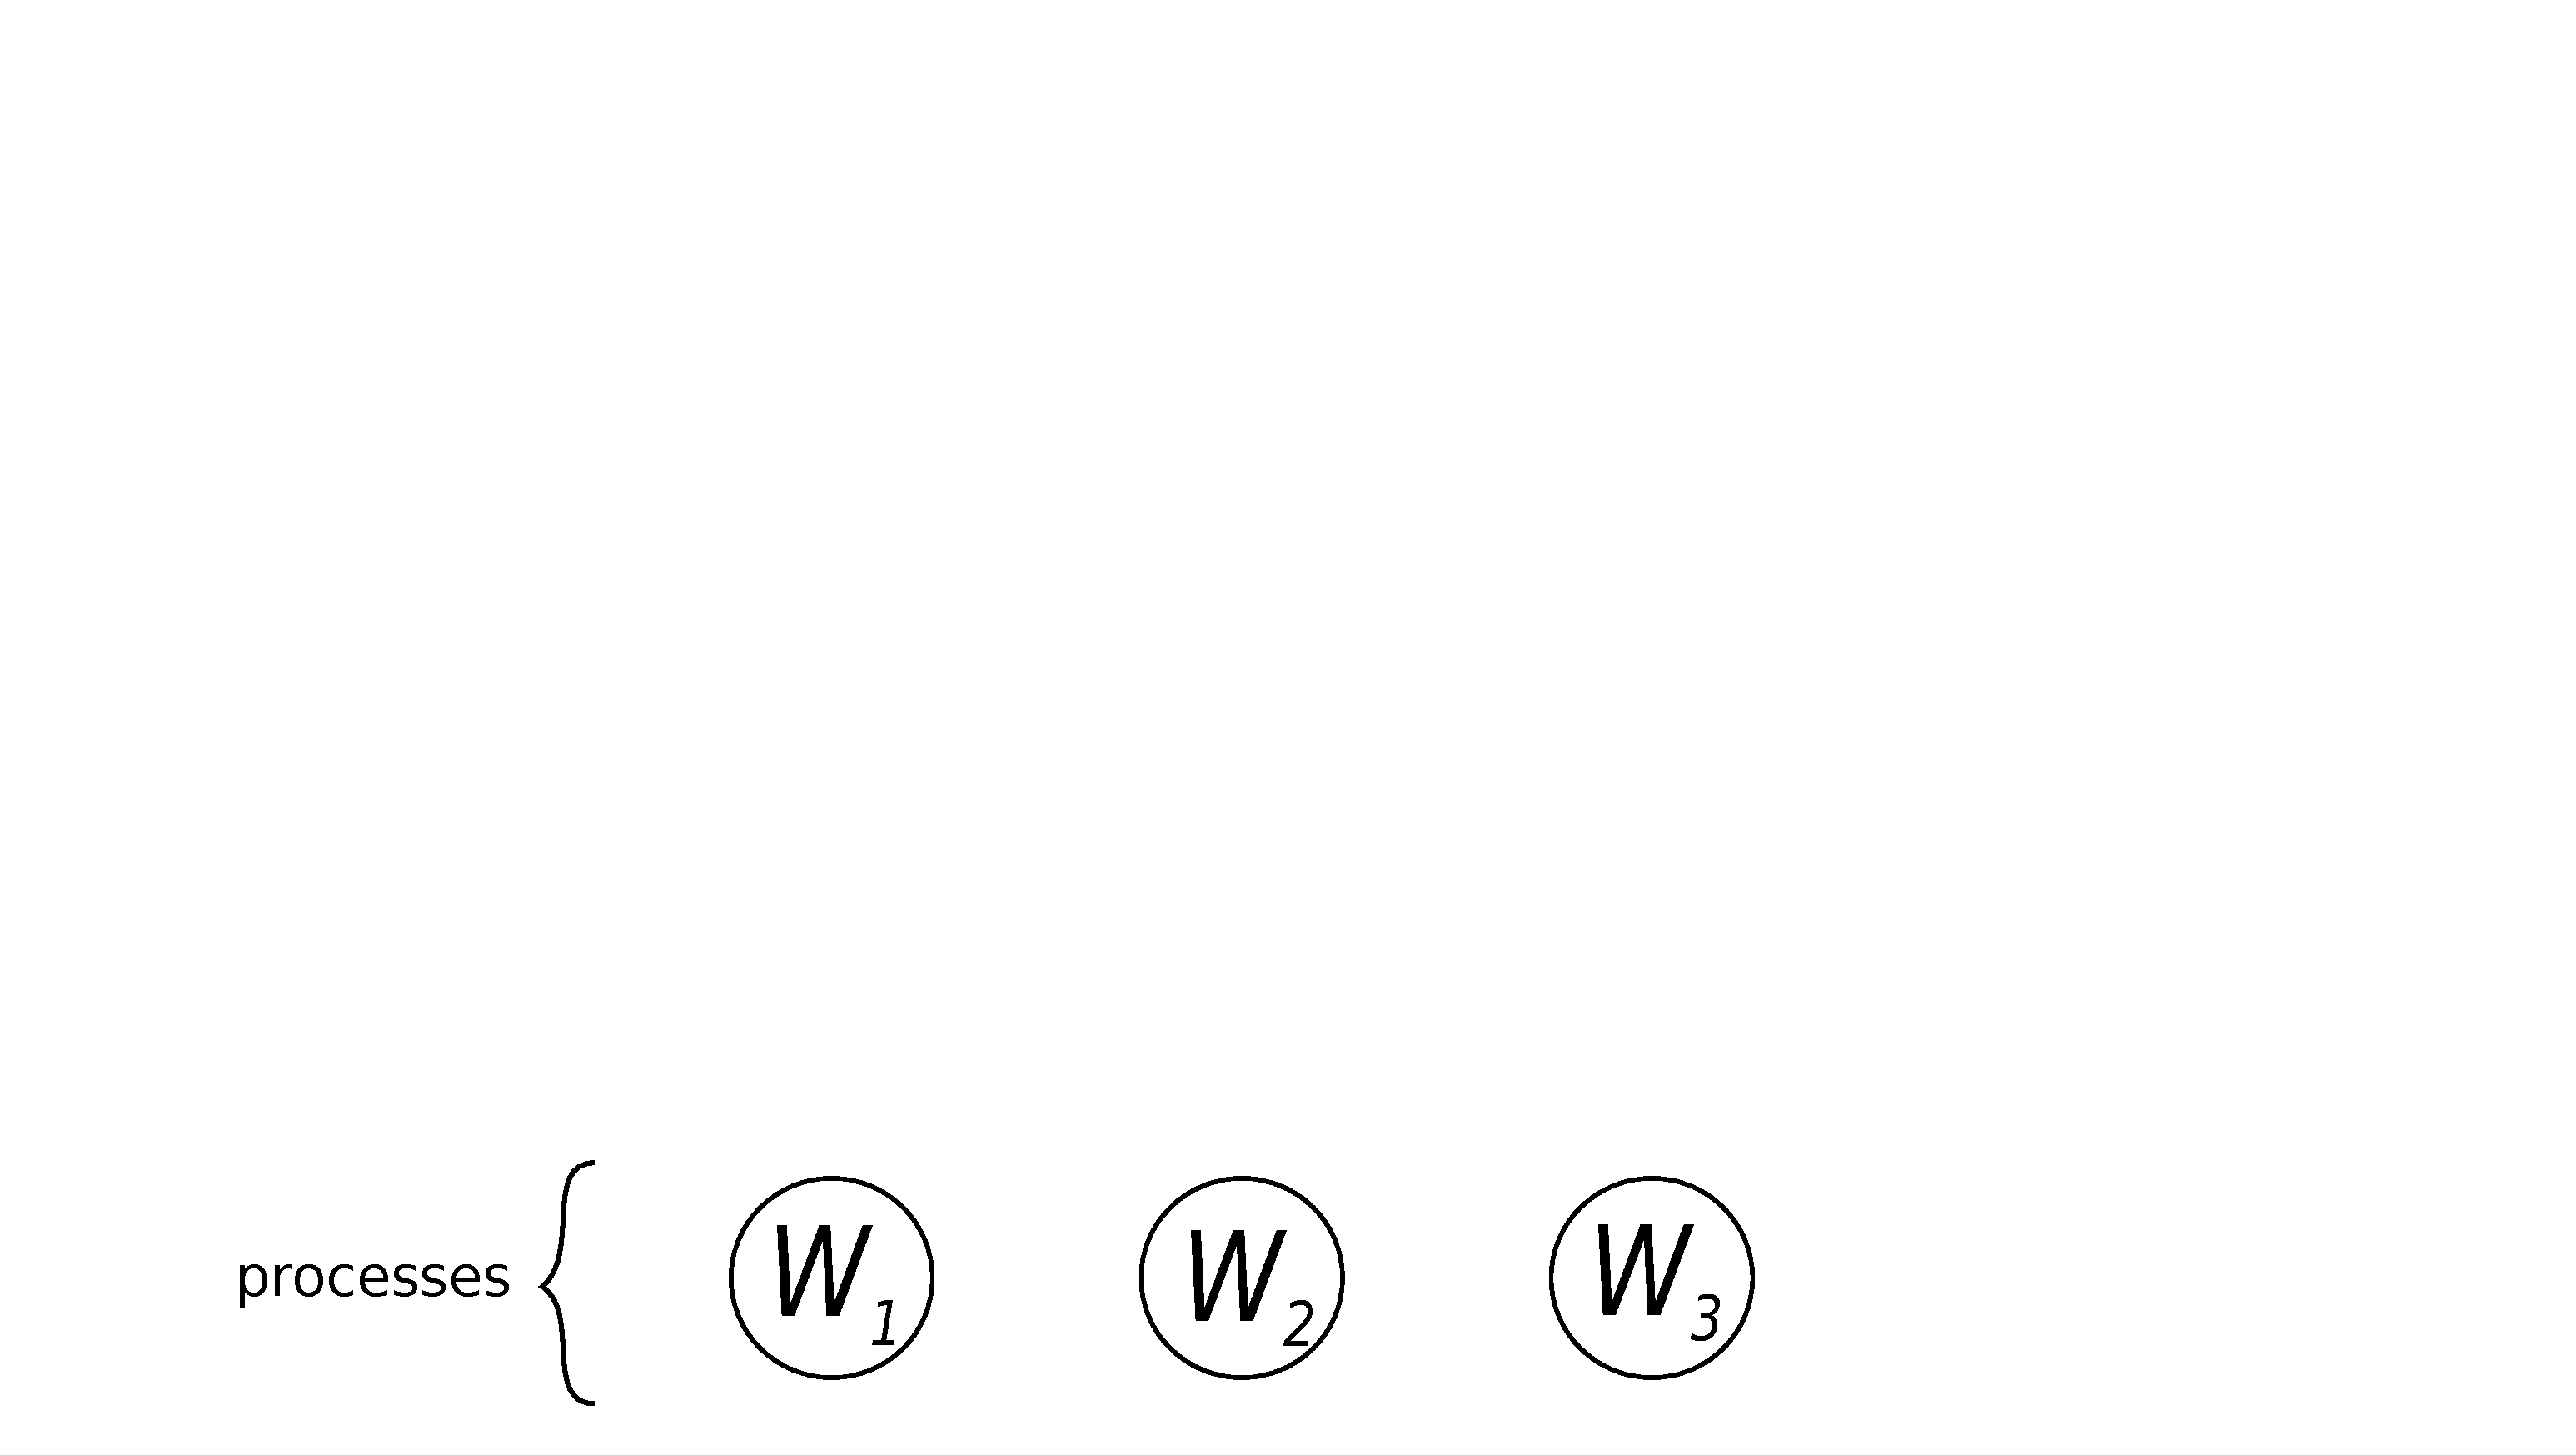
\includegraphics[width=.8\textwidth]{figures/MPST1.pdf}}%
  \only<2>{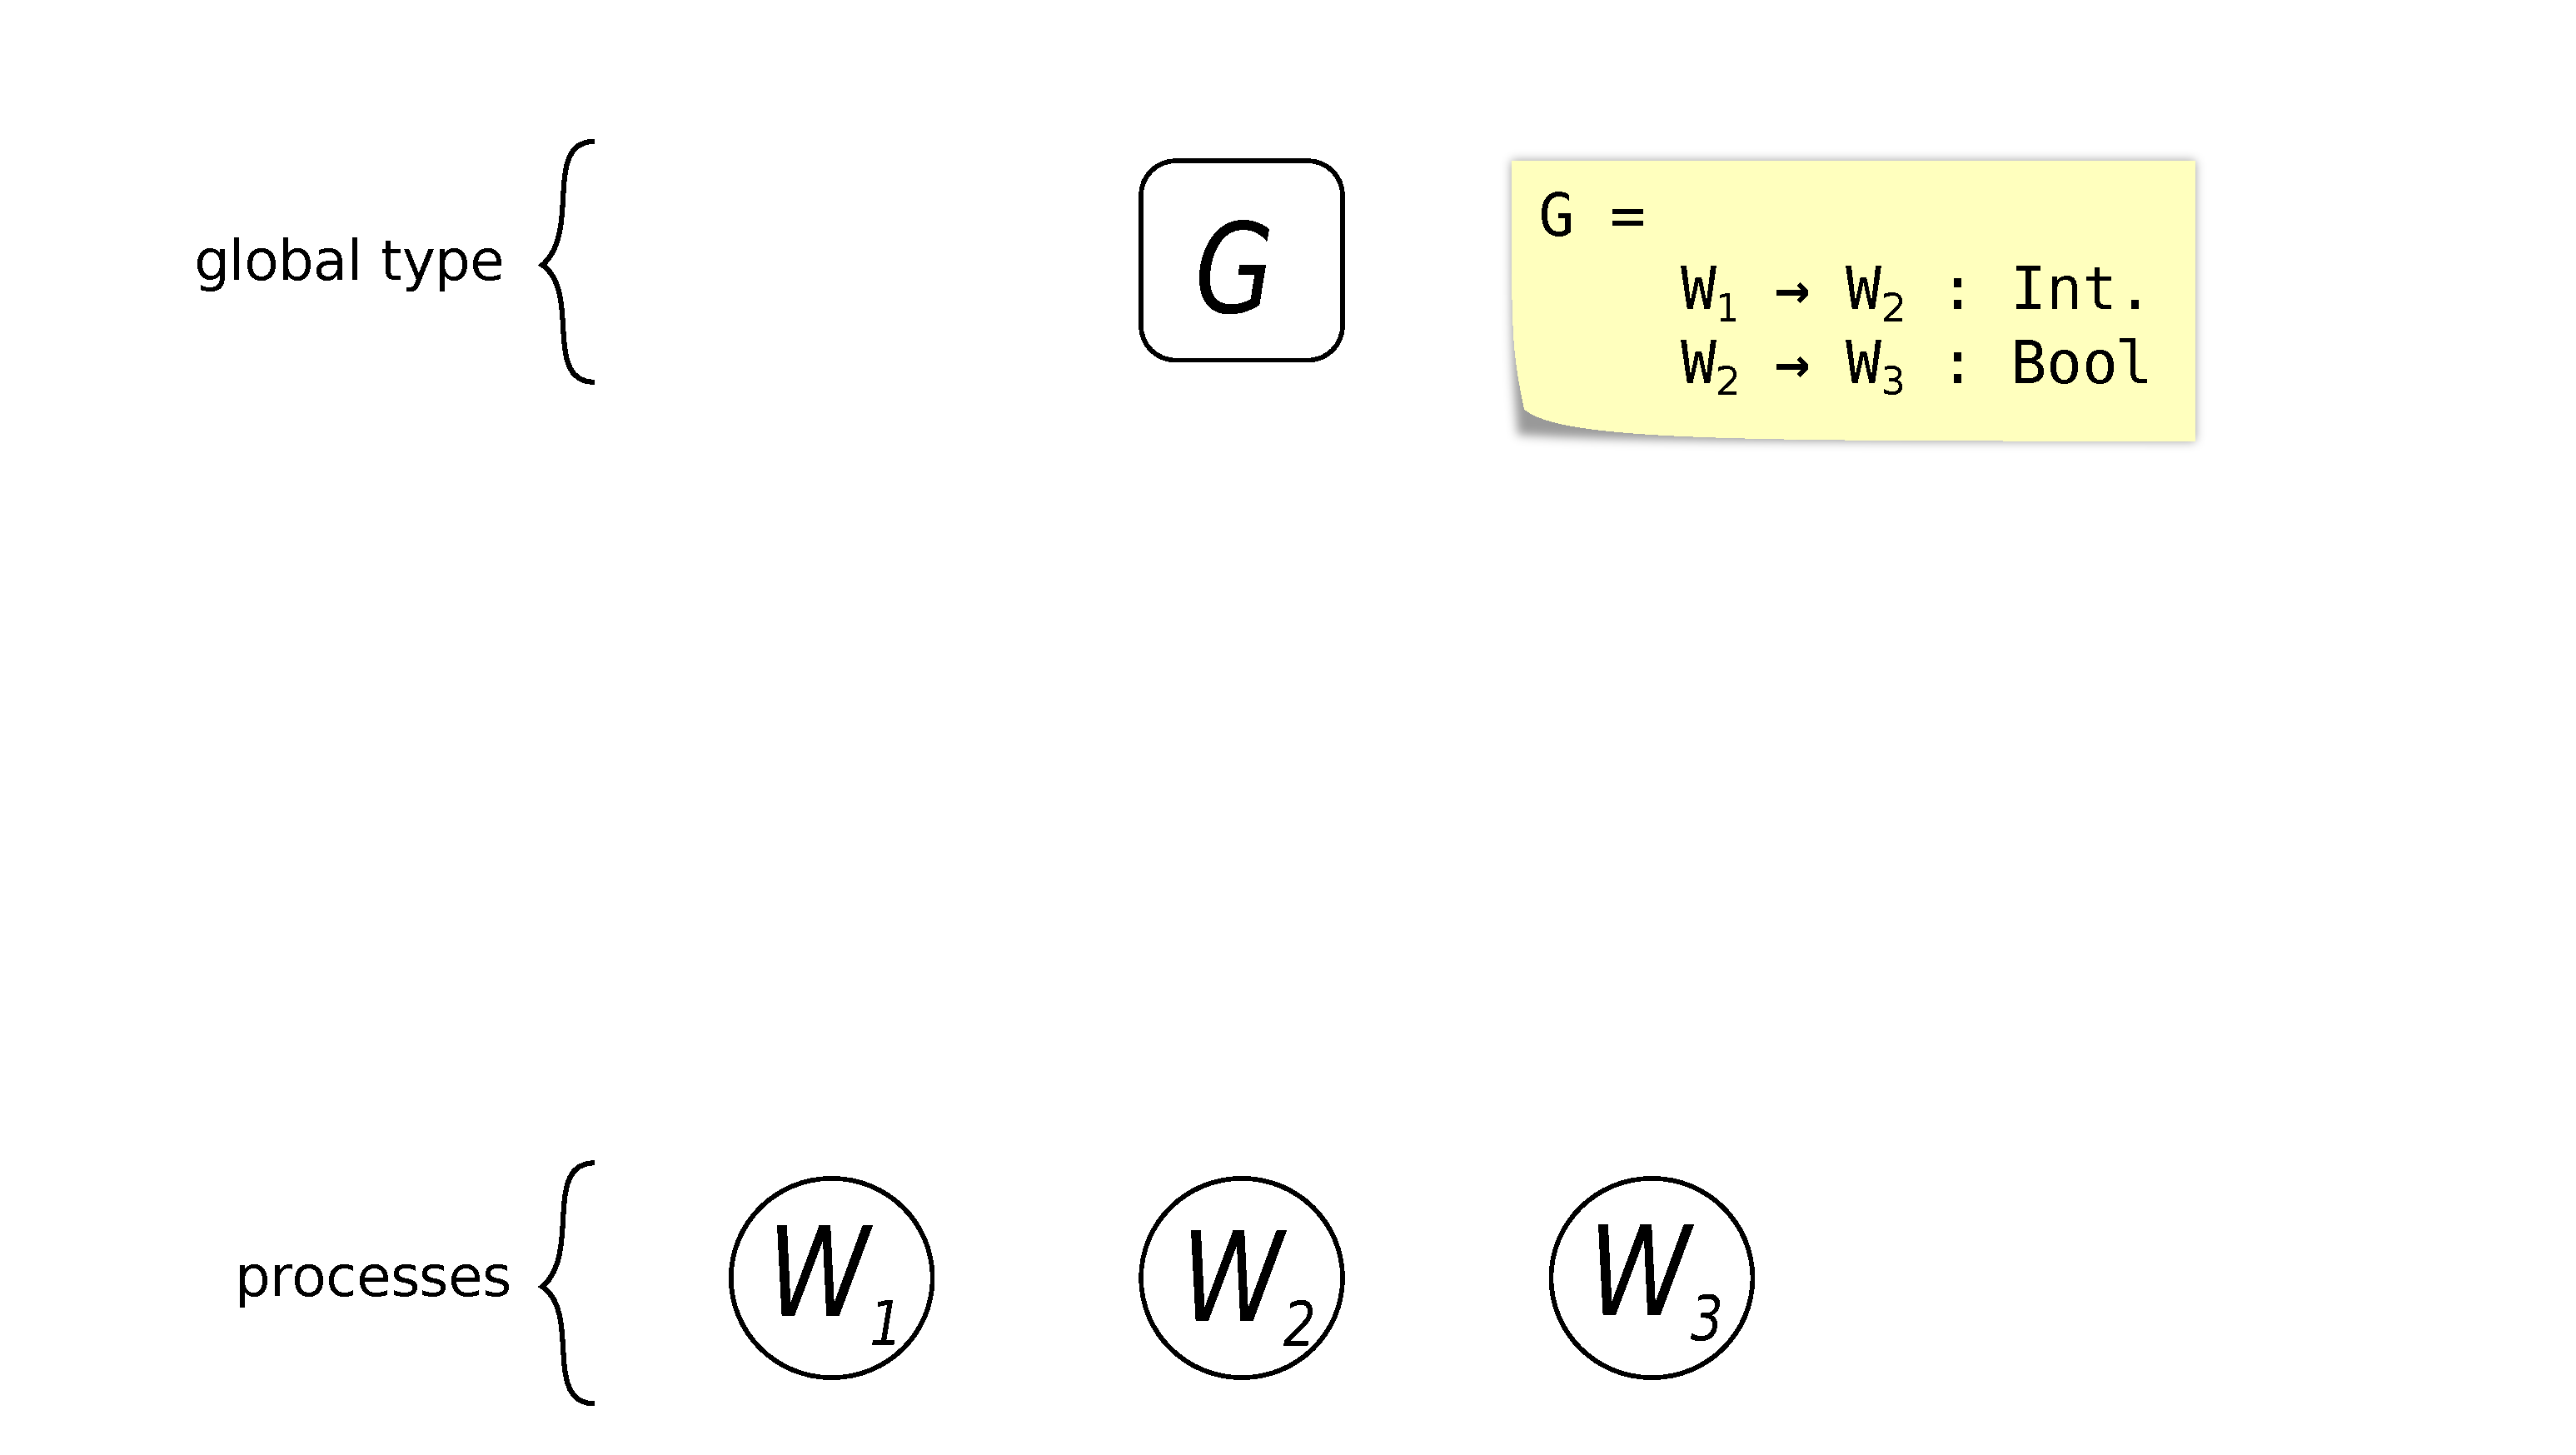
\includegraphics[width=.8\textwidth]{figures/MPST2.pdf}}%
  \only<3>{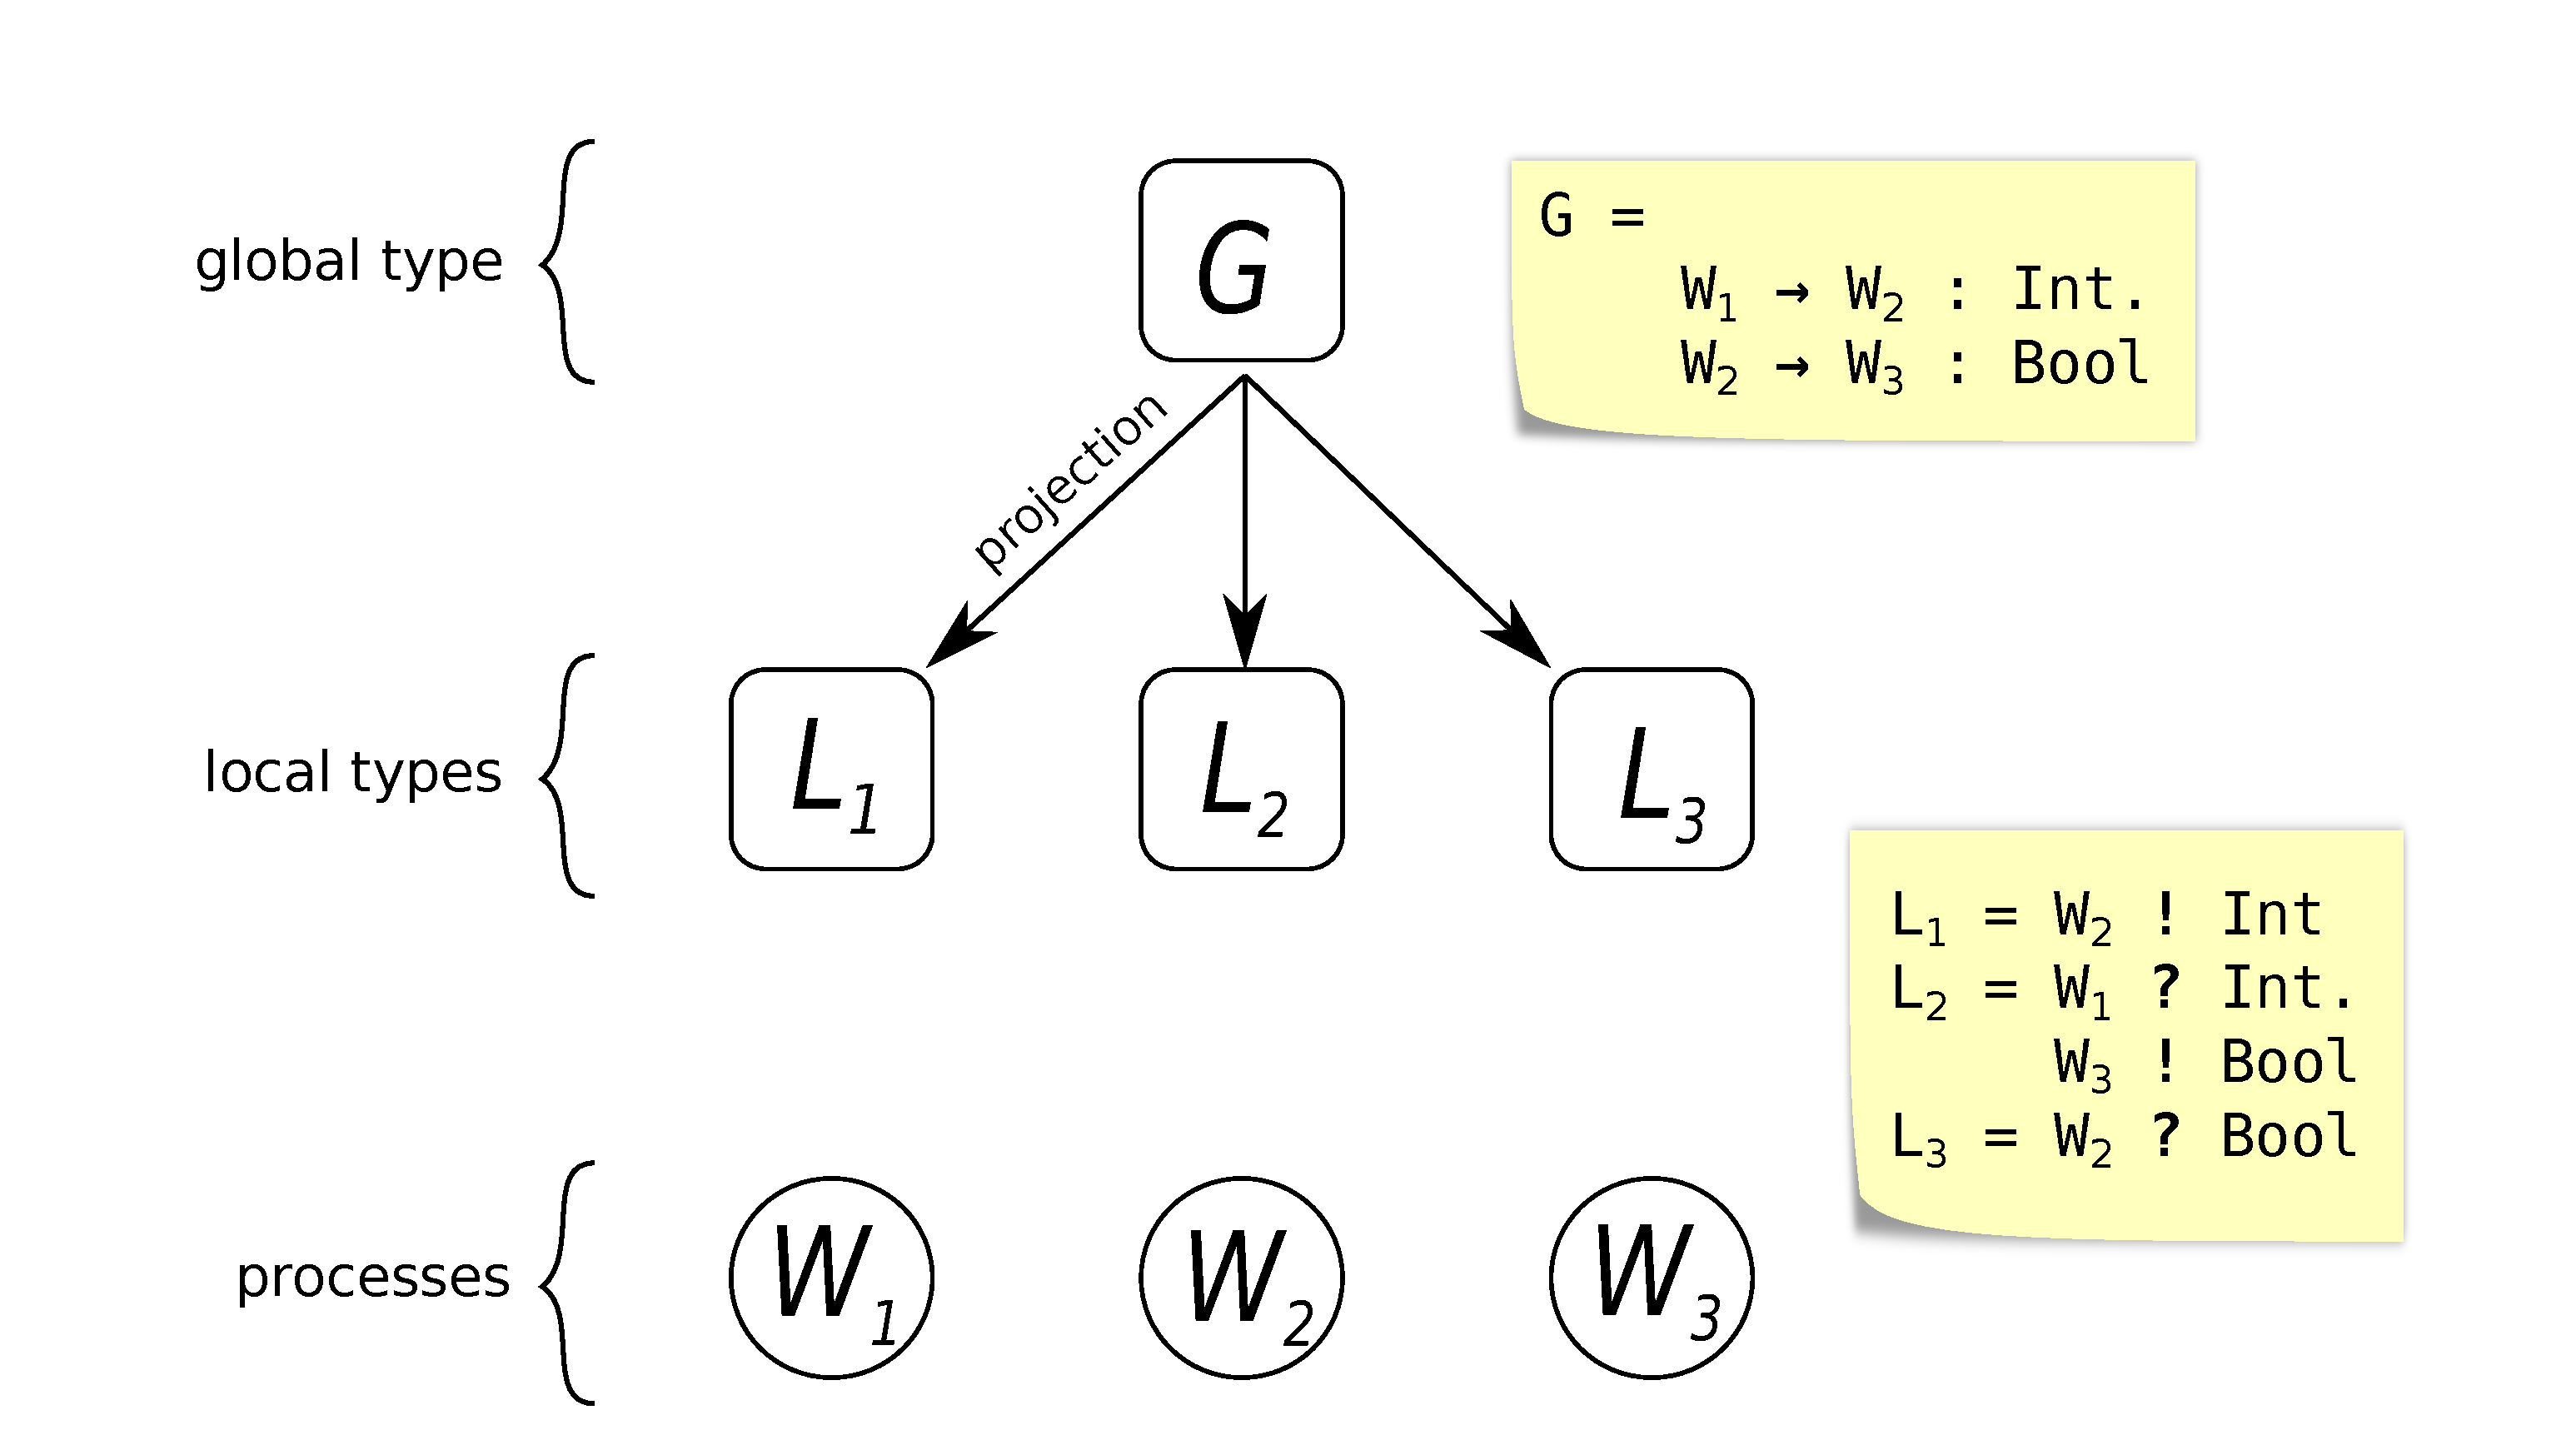
\includegraphics[width=.8\textwidth]{figures/MPST3.pdf}}%
  \only<4>{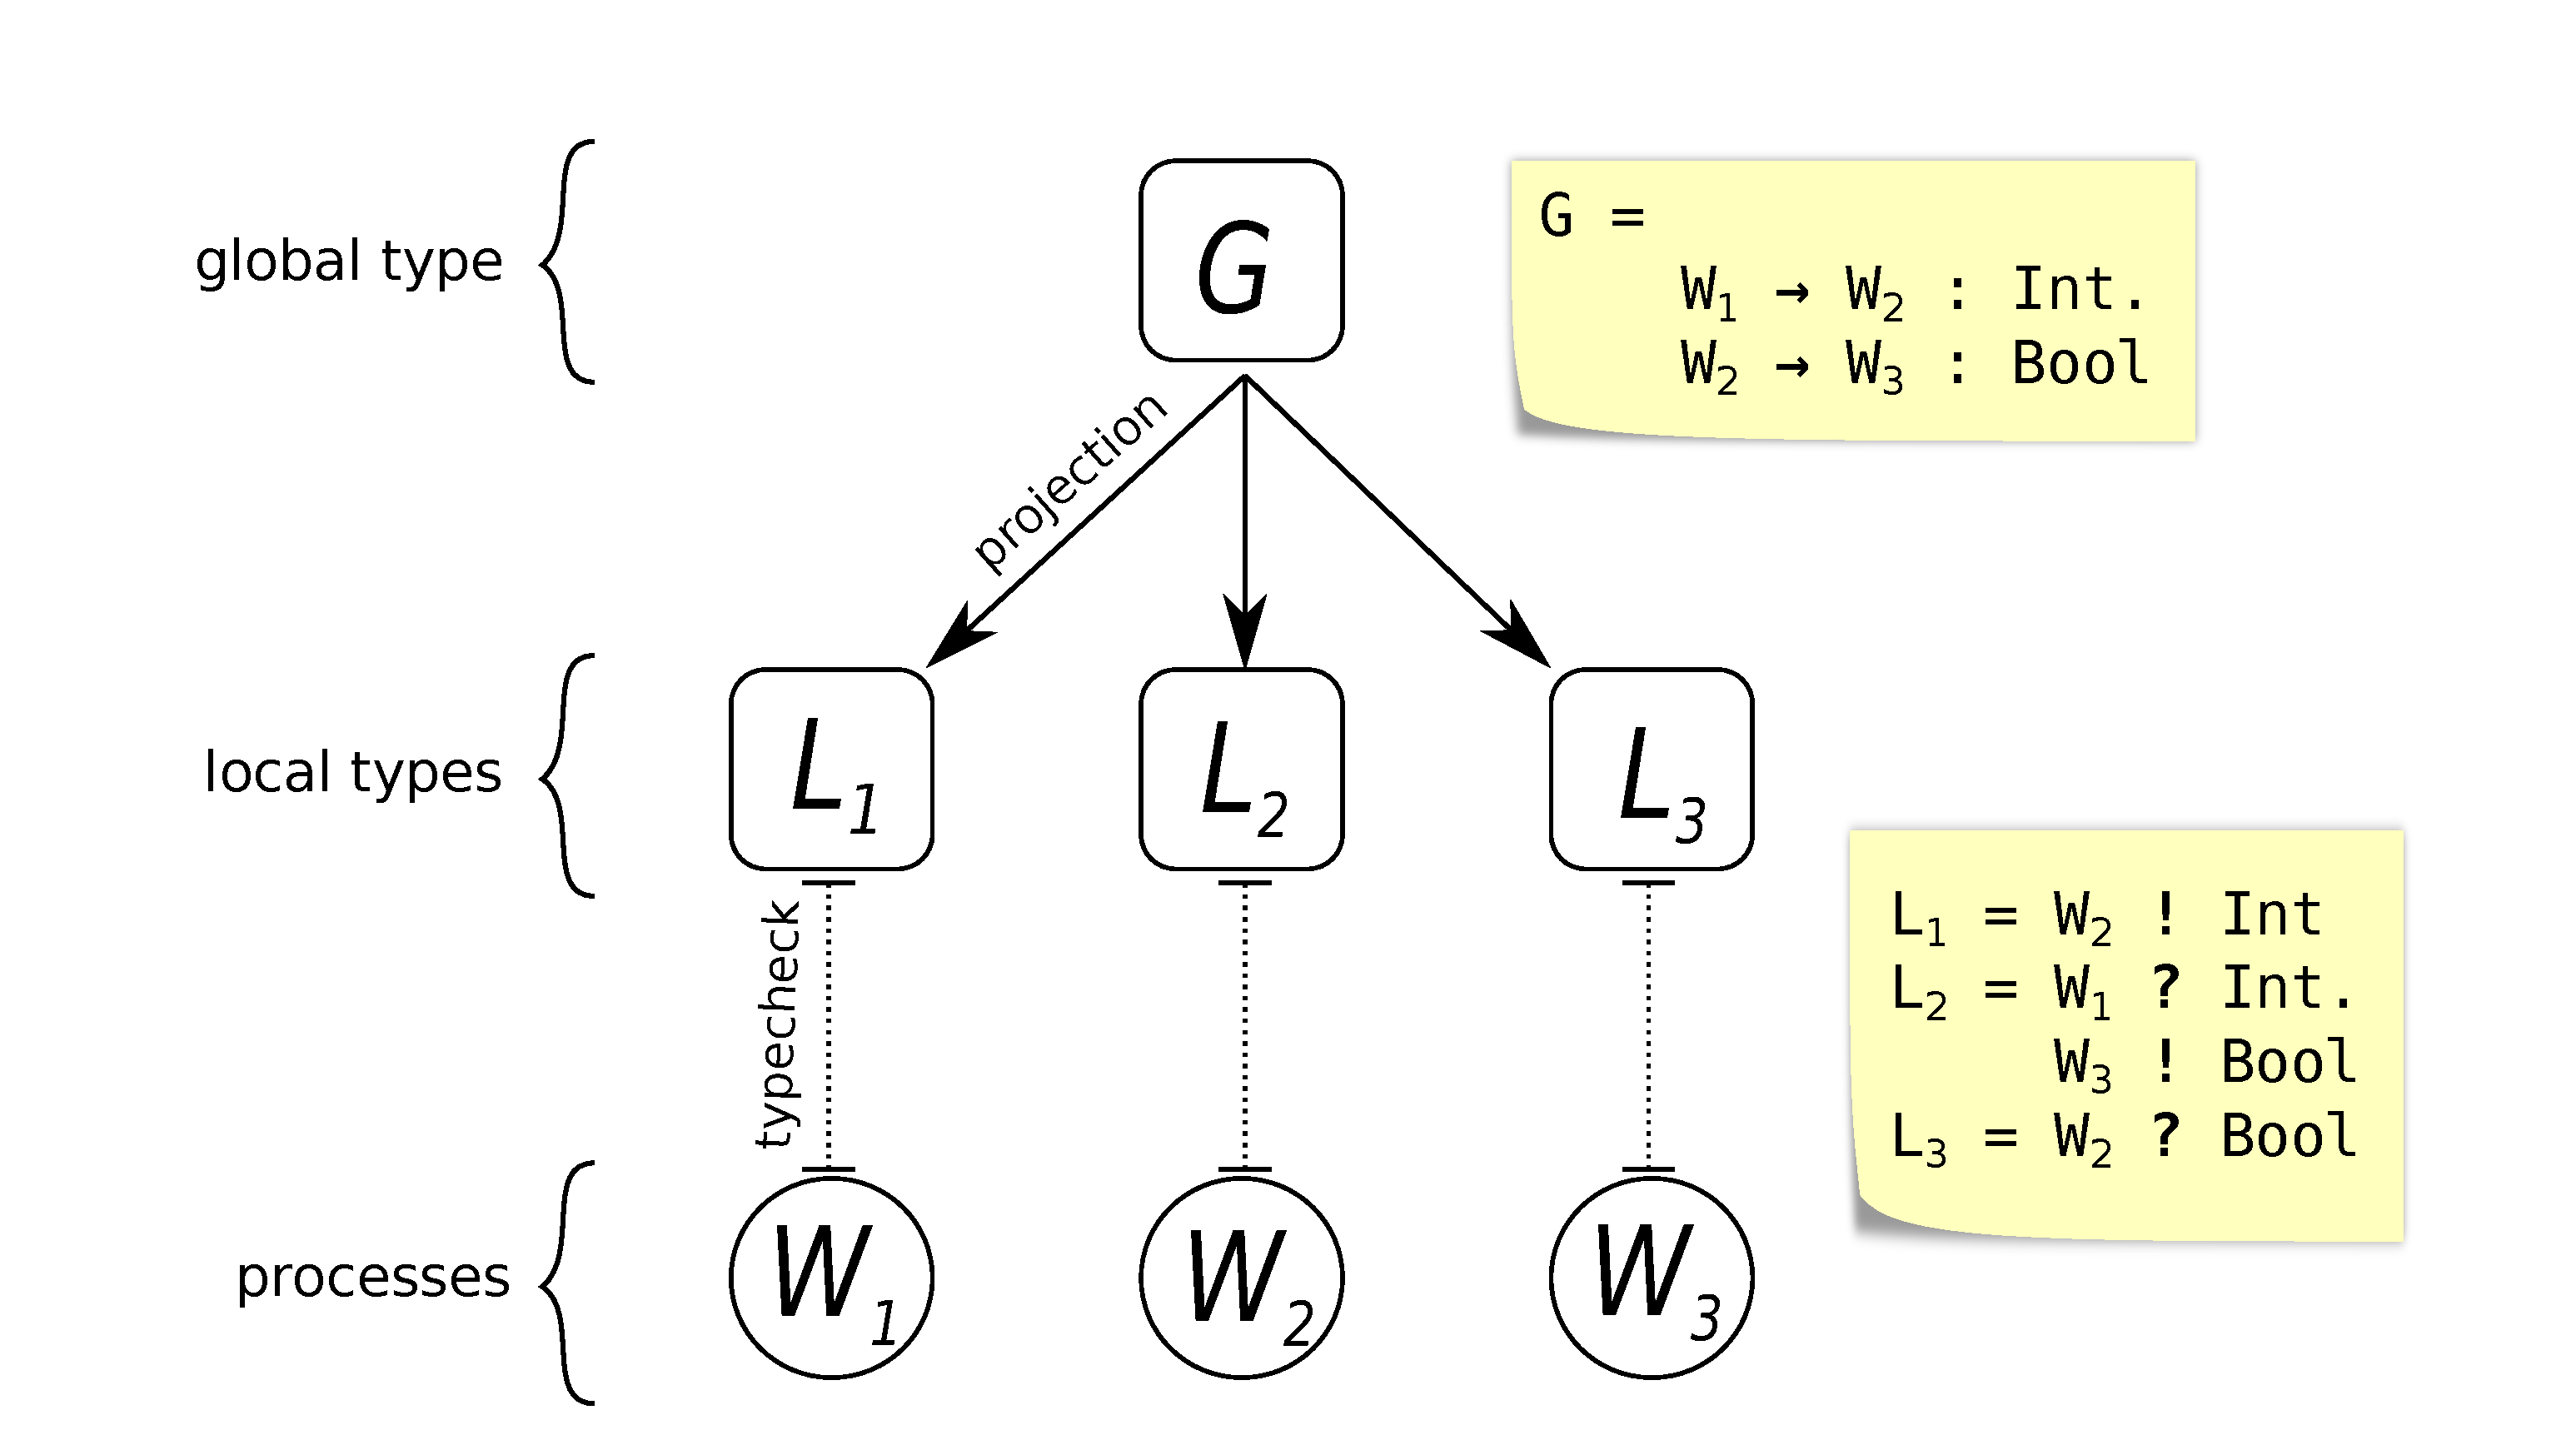
\includegraphics[width=.8\textwidth]{figures/MPST4.pdf}}%
  \only<5>{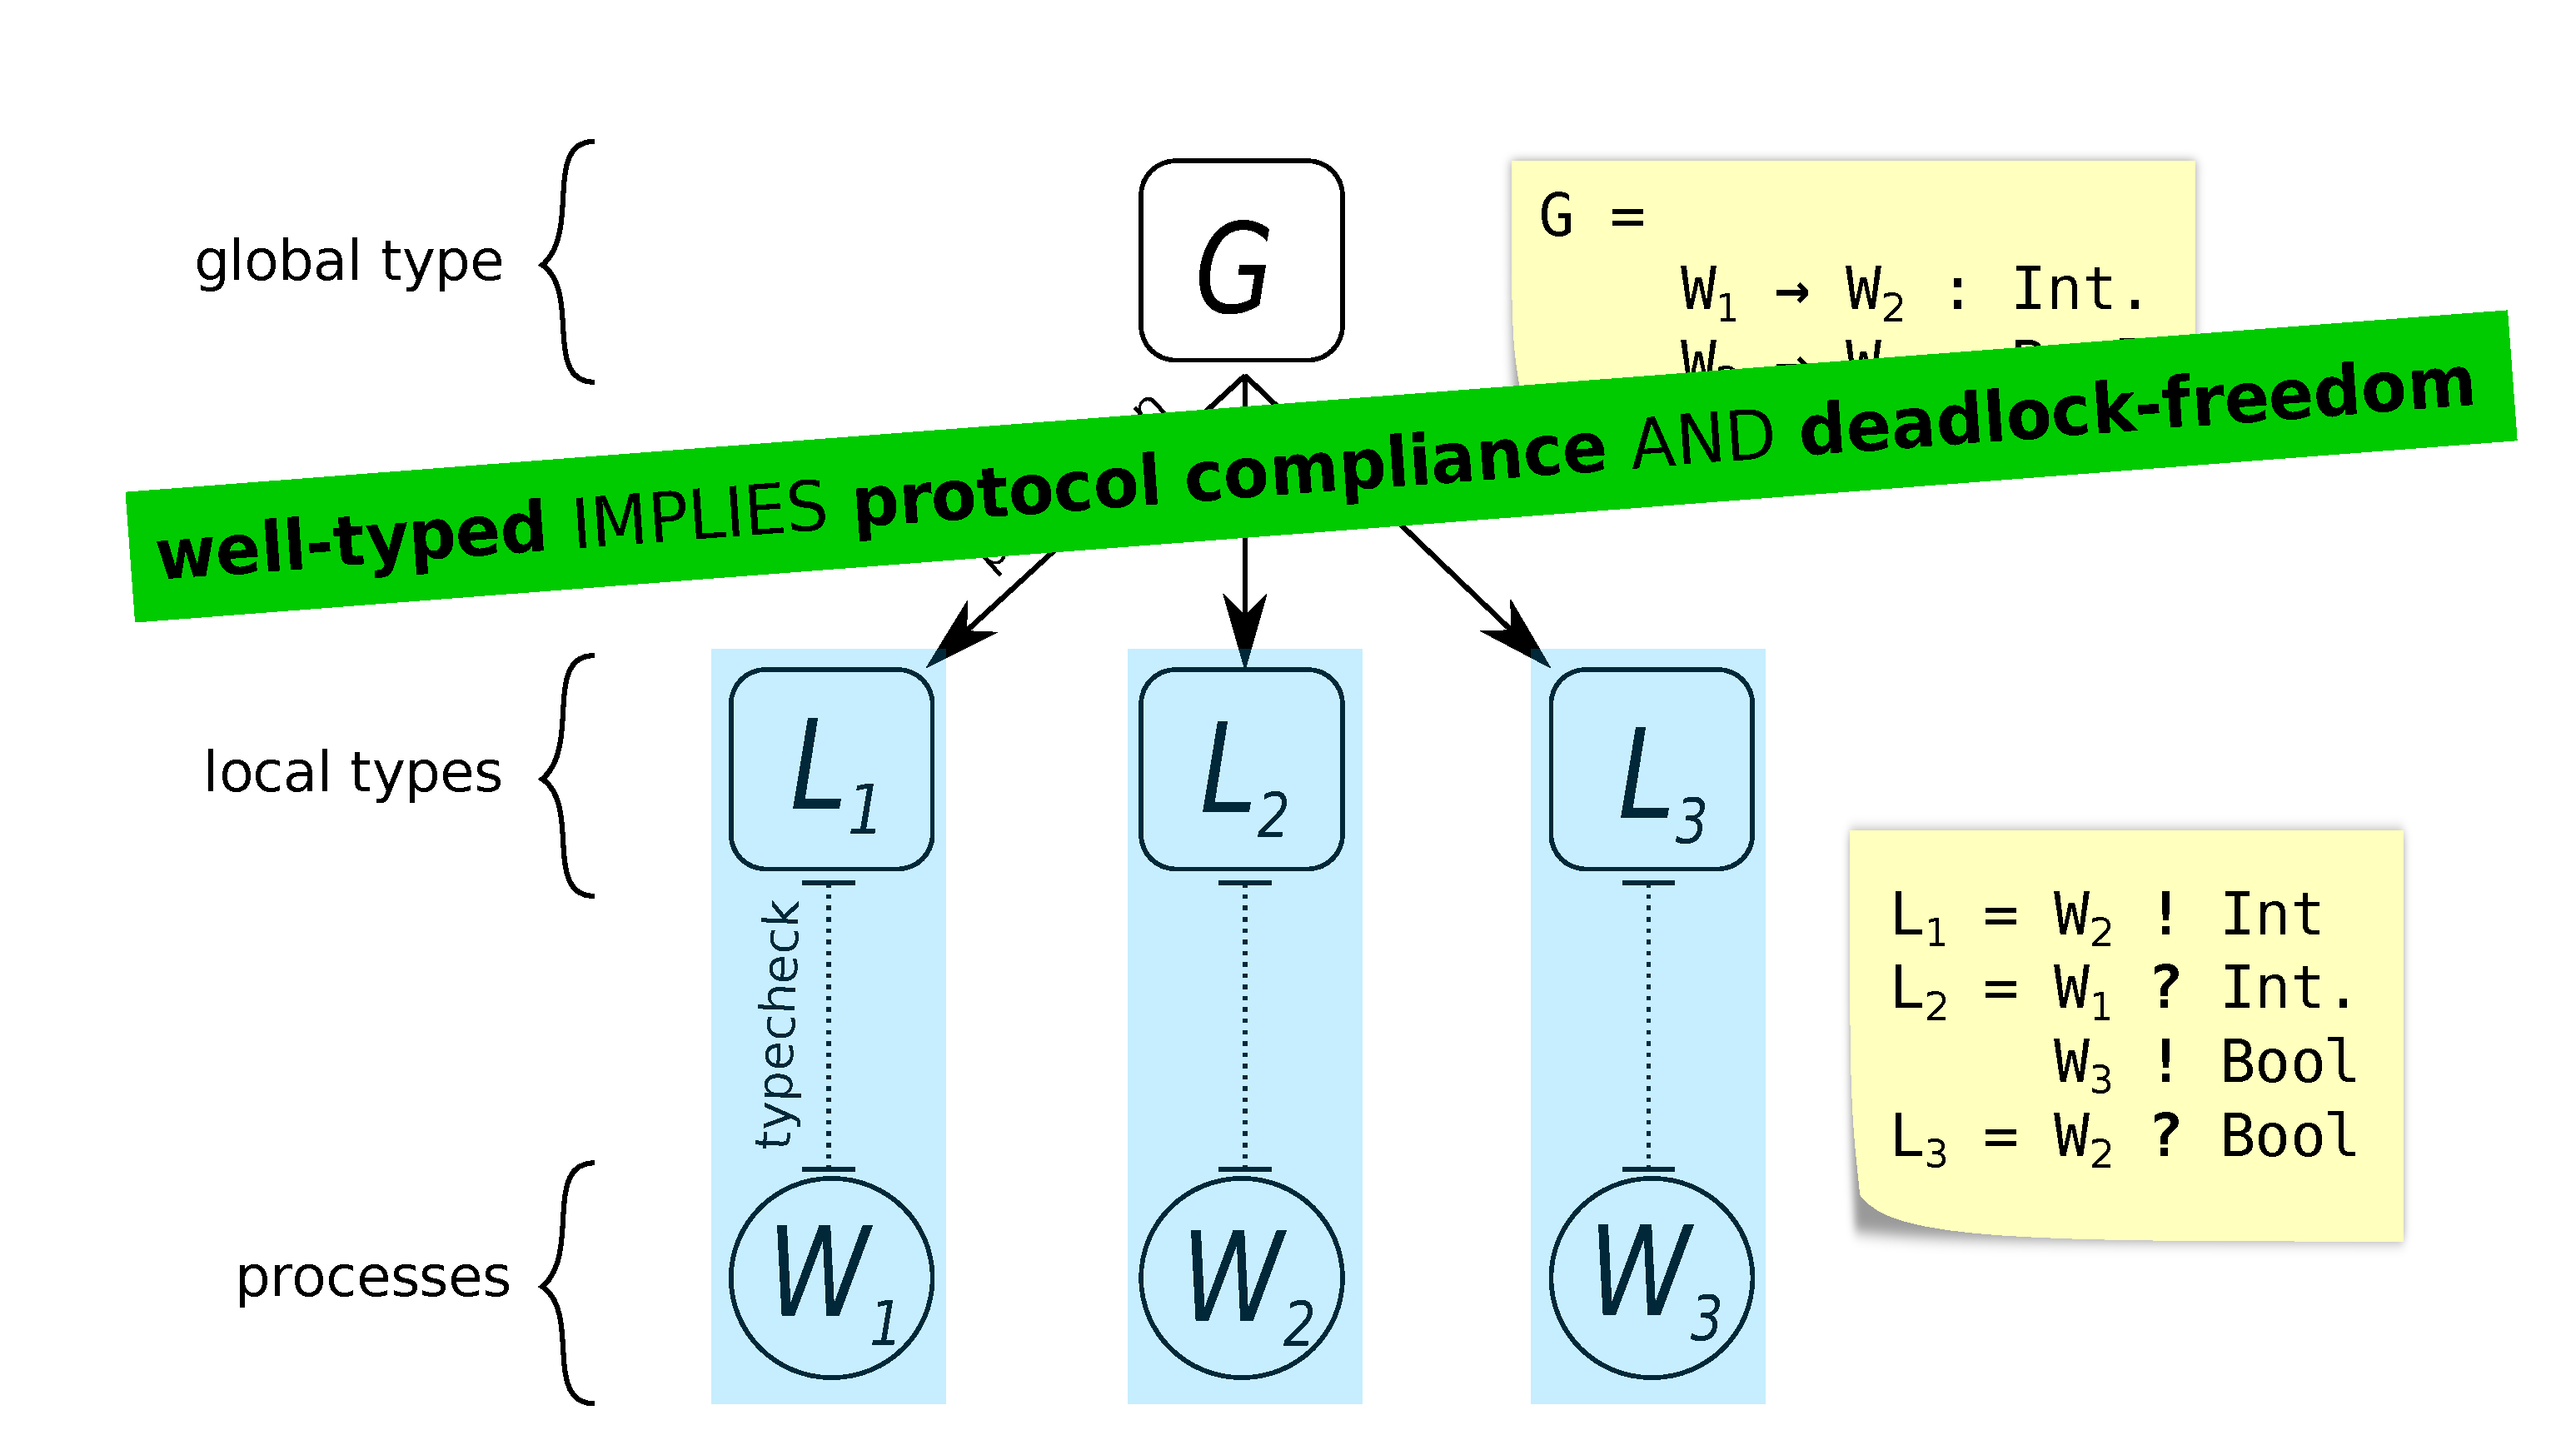
\includegraphics[width=.8\textwidth]{figures/MPST5.pdf}}
  \end{center}
\end{frame}

\begin{frame}{Global and Local Types}
\begin{displaymath}
  \begin{array}{lrcll}
    \text{Roles} &  &  & \Rp, \Rq, \ldots &  \\\\
    \text{Sorts} & \expt{S} & \mathrel{:=} & \sbool \mid \snat \mid \cdots & \text{Basic data types.} \\\\
    \text{Global Types} & \globalt{G} & \mathrel{:=}
    & \gmsg \Rp \Rq {{\gmsgbr {\lbl_i} {S_i} {G_i}}_{i\in I}} & \text{Message communication.} \\
    & & \mid & \grecur X G & \text{Recursion.} \\
    & & \mid & \pvar X & \text{Recursion variable.} \\
    & & \mid & \gfinish & \text{End of protocol.} \\\\
    \text{Local Types} & \localt{L} & \mathrel{:=}
    & \lsend \Rp {{\lmsgbr {\lbl_i} {S_i} {L_i}}_{i\in I}} & \text{Send message.} \\
    & & \mid & \lrecv \Rq {{\lmsgbr {\lbl_i} {S_i} {L_i}}_{i\in I}} & \text{Receive message.} \\
    & & \mid & \lrecur X G & \text{Recursion.} \\
    & & \mid & \pvar X & \text{Recursion variable.} \\
    & & \mid & \lfinish & \text{End of protocol.} \\
  \end{array}
\end{displaymath}

\end{frame}

\begin{frame}{Projection}

\begin{displaymath}
  \begin{array}{c}
\gproj{\gmsg \Rp \Rq {{\gmsgbr {\lbl_i} {S_i} {G_i}}_{i\in I}}}{\Rr} =
\left\{%
\begin{array}{l l}
\lsend \Rq {{\lmsgbr {\lbl_i} {S_i} {\gproj{G_i}{\Rr}}}_{i\in I}} & (\Rr = \Rp \wedge \phantom{\Rr = \Rq} \wedge \Rp \neq \Rq) \\
\lrecv \Rp {{\lmsgbr {\lbl_i} {S_i} {\gproj{G_i}{\Rr}}}_{i\in I}} & (\phantom{\Rr = \Rp} \wedge \Rr = \Rq \wedge \Rp \neq \Rq) \\
\lmerge_{i \in I}(\gproj{G_i}{\Rr}) & (\Rr \neq \Rp \wedge \Rr \neq \Rq \wedge \Rp \neq \Rq) \\
\end{array}
\right.
\\[1cm]
\gproj{\grecur X G}{\Rr} =
\left\{%
\begin{array}{l l}
  \lrecur X {\gproj{G}{\Rr}} & (\Rr \in G) \\
  \lfinish & (\Rr \not\in G)
\end{array}
\right.
\hspace{1cm}
\gproj{\pvar X}{\Rr} = \pvar X
\hspace{1cm}
\gproj{\gfinish}{\Rr} = \lfinish
  \end{array}
\end{displaymath}

\noindent\makebox[\linewidth]{\rule{\columnwidth}{0.4pt}}

\uncover<2->{%
\begin{displaymath}
  \begin{array}{c}
    \begin{array}{l}
\lrecv \Rp {{\lmsgbr {\lbl_i} {S_i} {L_i}}_{i\in I}}
\mathbin{\lmerge}
\lrecv \Rp {{\lmsgbr {\lbl_j} {S_j} {L'_j}}_{j\in J}}
\\\quad
= \lrecv \Rp {{\lmsgbr {\lbl_i} {S_i} {L_i}}_{i\in I\setminus J}
  \cup {\lmsgbr {\lbl_j} {S_j} {L'_j}}_{j\in J\setminus I}
\cup {\lmsgbr {\lbl_i} {S_i} {L_i \mathbin{\lmerge} L'_i}}_{i\in I \cap J}}
\\[.5cm]
\lsend \Rp {{\lmsgbr {\lbl_i} {S_i} {L_i}}_{i\in I}}
\mathbin{\lmerge}
\lsend \Rp {{\lmsgbr {\lbl_i} {S_i} {L'_i}}_{i\in I}}
=
\lsend \Rp {{\lmsgbr {\lbl_i} {S_i} {L_i \lmerge L'_i}}_{i\in I}}
\\[.5cm]
\lrecur X L \mathbin{\lmerge} \lrecur X L' = \lrecur X (L \mathbin{\lmerge} L')
\hspace{1cm}
L \mathbin{\lmerge} L = L
\end{array}
  \end{array}
\end{displaymath}
}
  \Put(40,290){%
    \begin{onlyenv}<3>
    \begin{minipage}{.86\columnwidth}
    \begin{infobox}
      \Large
      \textbf{It gets complicated very quickly!}
    \end{infobox}
    \end{minipage}
    \end{onlyenv}
  }
\end{frame}

\begin{frame}{What is the point of $\lmerge$?}
  Consider the following protocol

  -- {\small this is similar to the behaviour of the previous Go code snippet:}

  \begin{displaymath}
    \grecur X {
\gmsg \Rp \Rq {\left\{%
  \begin{array}{l@{}l}
   \dlbl{\mathsf{REQ}}(\snat) &. \gmsg \Rq \Rr {\dlbl{\mathsf{REQ}}(\sbool). \pvar{X}} \\
   \dlbl{\mathsf{END}}() &. \gmsg \Rq \Rr {\dlbl{\mathsf{END}}(). \pfinish}
  \end{array}
   \right\}}}
  \end{displaymath}

  \vspace{1cm}
  \uncover<2->{%
    Projecting $\Rr$
  \begin{displaymath}
    \begin{array}{l}
    \lrecur X {
      (\lrecv \Rq {\dlbl{\mathsf{REQ}}(\sbool). \pvar{X}})
        \mathbin{\lmerge}
      (\lrecv \Rq {\dlbl{\mathsf{END}}(). \lfinish})
   }
    \\[.3cm] \qquad =
    \uncover<3>{%
    \lrecur X {
\lrecv \Rq {\left\{%
  \begin{array}{l@{}l}
   \dlbl{\mathsf{REQ}}(\sbool) &. \pvar{X} \\
   \dlbl{\mathsf{END}}() &. \pfinish
  \end{array}
   \right\}}}
    \end{array}
  \end{displaymath}
  }}

\end{frame}


\begin{frame}{Processes and Typing}

\begin{displaymath}
  \begin{array}{lrcll}
    \text{Process} & \proc{P} & \mathrel{:=} & \psend p \lbl e P & \text{Send a message.} \\
    & & \mid & \precv i I {\precbr p {\lbl_i} {x_i} {P_i}} & \text{Receive a message.} \\
    & & \mid & \pif e P {P'} & \text{Conditional process.} \\
    & & \mid & \precur X P & \text{Recursive process.} \\
    & & \mid & \pvar X & \text{Recursion variable.} \\
    & & \mid & \pfinish & \text{Inactive process.} \\
  \end{array}
\end{displaymath}

\end{frame}

\begin{frame}{Process Typing (simplified)}
  Once we have local types, process typing is simple:
  \vspace{.4cm}

\begin{displaymath}
  \begin{array}{c}
  \infer[T-SEND]
  { \loft \Gamma P {L_i} \and \toft \Gamma e S_i \and i \in I}
  {\loft \Gamma {\psend \Rq {\lbl_i} e P} (\lsend \Rp {{\lmsgbr {\lbl_i} {S_i} {L_i}}_{i\in I}})}
  \hspace{1cm}
  \infer[T-RECV]
  { \loft {\Gamma , {\pvar{x_i}} : {\expt{S_i}}} {P_i} {L_i} \and \forall i \in I}
  {\loft \Gamma {\precv i I {\precbr p {\lbl_i} {x_i} {P_i}}} (\lrecv \Rp {{\lmsgbr {\lbl_i} {S_i} {L_i}}_{i\in I}})}
  \end{array}
\end{displaymath}

\end{frame}

\begin{frame}{Problems with Classic Formulation}
  \begin{enumerate}
    \item \textbf{Too syntactic:}
      \begin{itemize}
        \item Processes and local types must align
        \item Too restrictive, rules out correct processes
        \item \ldots
      \end{itemize}
    \item \textbf{Unnecessarily complex:}
      \begin{itemize}
        \item Hard to implement/mechanise, e.g.:
          \begin{itemize}
            \item Use of runtime coinductive global types: Our PLDI 2021 paper
            \item Complex graph-based representation of MPST: Jacobs et al. (2022)
            \item Graph-based reasoning and decision procedure for the equality
              of recursive types: Tirore et al. (2023)
          \end{itemize}
        \item Hard to extend
      \end{itemize}
    \item \textbf{Imprecise} about the uses of coinduction
  \end{enumerate}
\end{frame}

\begin{frame}{Example of Imprecision in Classic MPST}
  \boxed{\text{``We identify $\grecur X G$ with $[\grecur X G / \pvar{X}] \globalt{G}$''}}

  \vspace{.4cm}

  This is a common statement in proofs about MPST, which clearly specifies an equirecursive formulation, but...
  \begin{enumerate}
    \item The rules still refer to open global types with variables $\pvar{X}$
    \item The rules specify when and how to unfold $\grecur X G$ -- if we are using equirecursion, $\grecur{}{}$ should not be in the syntax ouf our language!
  \end{enumerate}

  \vspace{.4cm}
  Moreover, this ``identification'' of a global type and its unfolding is not powerful enough. E.g.
  \[
    \gmsg \Rp \Rq {\gmsg {\Rp'} {\Rq'} G} \neq \gmsg {\Rp'} {\Rq'} {\gmsg \Rp \Rq G}
  \]
  This forces the use of tedious syntactic proofs about how the swapping of unrelated actions does not affect the protocol.
\end{frame}

\begin{frame}{A Few Attempts at Simplifying the Theory}

    \begin{minipage}{.86\columnwidth}
    \begin{sticky}
  
\includegraphics[width=\textwidth]{figures/less-is-more.pdf}
    \end{sticky}
    \end{minipage}

  \Put(40,40){%
    \begin{onlyenv}<2->
    \begin{minipage}{.86\columnwidth}
    \begin{sticky}
  
\includegraphics[width=\textwidth]{figures/less-is-more-revisite.pdf}
    \end{sticky}
    \end{minipage}
    \end{onlyenv}
   }

\end{frame}

\begin{frame}
  
\includegraphics[width=\columnwidth]{figures/xkcd-standards.png}
  \href{https://xkcd.com/927/}{https://xkcd.com/927/}
\end{frame}


\begin{frame}{Our Approach: Synthetic Typing}
    \begin{minipage}{.86\columnwidth}
    \begin{sticky}
  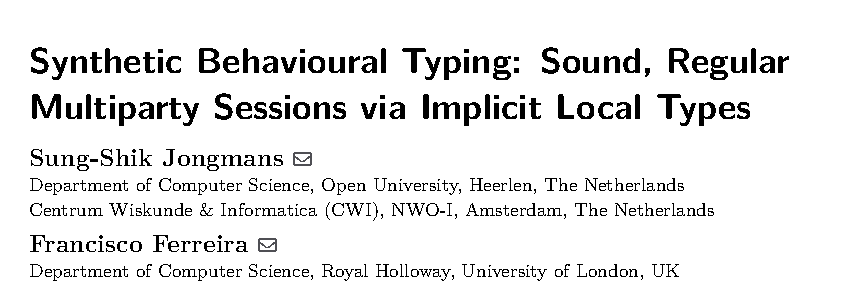
\includegraphics[width=\textwidth]{figures/fs-synthetic.pdf}
    \end{sticky}
    \end{minipage}

  \Put(40,140){%
    \begin{onlyenv}<2->
    \begin{minipage}{.86\columnwidth}
      \begin{greenbox}
        Goals:
        \begin{itemize}
          \item ``Free'' typing from being tied up to the syntax of local types.
          \item Avoid projection/merging/etc.
\item A formal description of equality
  between global types to replace informally equating global types to
  their unfolding.
          \item Well-formedness/deadlock-freedom is decided by typeability.
          \item Mechanisation in Agda.
        \end{itemize}
      \end{greenbox}
    \end{minipage}
    \end{onlyenv}
   }
\end{frame}


\begin{frame}
  \vfill
  \centering
  %\begin{beamercolorbox}[sep=8pt,center,shadow=true,rounded=true]{block}
  \begin{sticky}
    \usebeamerfont{title}
    {\normalfont \textbf{Towards Synthetic MPST (WIP)}}
    \par%
  \end{sticky}
  %\end{beamercolorbox}
  \vfill
\end{frame}

\begin{frame}{New (Synthetic) Core Typing Rules}
  \only<1>{%
  \blfootnote{Synthetic, in that $\globalt{G'}$ occurs only in the premise, not
    in the conclusion. $\globalt{G'}$ needs to be \emph{synthesised} by using
    the rules of the operational semantics of global types (Jongmans and Ferreira, 2023).}
\boxed{\textbf{New judgement}: \hspace{.2cm} $\poft \Gamma P G \Rp$}}
\vspace{.5cm}

{\scriptsize
\begin{displaymath}
  \begin{array}{c}
  \uncover<1-2>{%
  \infer[T-SEND]
  {\poft \Gamma P {G'} \Rp \and \greduce G {\annlbl \Rp \Rq {\lbl(\expt{S})}} {G'} \and
  \toft \Gamma e S}
  {\poft \Gamma {\psend \Rq \lbl e P} G \Rp}
  }

  \hspace{.6cm}

  \infer[T-RECV]
  {  \poft {\Gamma, {\pvar{x_i}} : {\expt{S_i}}} {P_i} {G'} \Rp \and
    \only<1-4>{\forall\; \greduce G {\annlbl \Rq \Rp {\lbl_i(\expt{S_i})}} {G'}}
    \only<5->{\boxed{\forall\; \greduce G {\annlbl \Rq \Rp {\lbl_i(\expt{S_i})}} {G'}}}
  }
  {\poft \Gamma {\precv i I {\precbr q {\lbl_i} {x_i} {P_i}}} G \Rp}

  \\[.4cm]

  \uncover<1-3>{%
  \infer[T-SKIP]
  { \poft \Gamma {P} {G'} \Rr  \and
    \forall \; \greduce G {\alpha} {G'}
    \; \text{s.t.} \; \Rr \not\in\mathsf{parts}(\alpha)
  }
  {\poft \Gamma P G \Rr}
  }
  \end{array}
\end{displaymath}
}
  \Put(40,320){%
    \begin{onlyenv}<2>
    \begin{minipage}{.86\columnwidth}
    \begin{infobox}
      \LARGE
      \textbf{What is wrong with these rules?}
    \end{infobox}
    \end{minipage}
    \end{onlyenv}
    \begin{onlyenv}<3>
    \begin{minipage}{.86\columnwidth}
    \begin{infobox}
      \LARGE
      \textbf{Hint: the problem is in these rules}
    \end{infobox}
    \end{minipage}
    \end{onlyenv}
    \begin{onlyenv}<4>
    \begin{minipage}{.86\columnwidth}
    \begin{infobox}
      \LARGE
      \textbf{Hint 2: the problem is the same in both rules, let's focus on this one}
    \end{infobox}
    \end{minipage}
    \end{onlyenv}
    \begin{onlyenv}<5>
    \begin{minipage}{.86\columnwidth}
    \begin{infobox}
      \LARGE
      \textbf{What happens if $\globalt{G}$ does not allow $\Rp$ to receive from $\Rq$?}
    \end{infobox}
    \end{minipage}
    \end{onlyenv}
    \begin{onlyenv}<6>
    \begin{minipage}{.86\columnwidth}
    \begin{infobox}
      \LARGE
      \textbf{This was a ``rookie'' mistake ... We cannot allow rules to be vacuously true!}
    \end{infobox}
    \end{minipage}
    \end{onlyenv}
  }
\end{frame}


\begin{frame}{(Hopefully) Fixed Typing Rules}
  \small
  Let $\mathcal{R}(\alpha, \globalt{G}) = \exists \globalt{G'}
  ,\; \greduce G {\alpha} {G'}$

  -- this means that an interaction $\alpha$ is
             ``ready'' (i.e. can happen) in $\globalt{G}$.

  Let $\mathcal{W}(\Rr, \globalt{G}) = \exists \alpha
  ,\; \mathcal{R}(\alpha, G) \wedge \Rr \not\in\mathsf{parts}(\alpha)$

  -- this means that $\Rr$ can ``wait'' for
    another (possibly unrelated) interaction in $\globalt{G}$.

\begin{displaymath}
  \begin{array}{@{}c@{}}
  \uncover<1,4->{%
  \infer[T-SEND]
  {\poft \Gamma P {G'} \Rp \and \greduce G {\annlbl \Rp \Rq {\lbl(\expt{S})}} {G'} \and
  \toft \Gamma e S}
  {\poft \Gamma {\psend \Rq \lbl e P} G \Rp}
  }

  \\[.4cm]

  \uncover<2,4->{%
  \infer[T-RECV]
    { \only<1-3>{\exists (j \in I), \mathcal{R}(\annlbl \Rq \Rp {\lbl_j(\expt{S_j})}, \globalt{G})}
      \only<4->{\boxed{\exists (j \in I), \mathcal{R}(\annlbl \Rq \Rp {\lbl_j(\expt{S_j})}, \globalt{G})}}
      \and
      \poft {\Gamma, {\pvar{x_i}} : {\expt{S_i}}} {P_i} {G'} \Rp \and
    \forall\; \greduce G {\annlbl \Rq \Rp {\lbl_i(\expt{S_i})}} {G'}
  }
  {\poft \Gamma {\precv i I {\precbr q {\lbl_i} {x_i} {P_i}}} G \Rp}
  }

  \\[.4cm]

  \uncover<3,4->{%
  \infer[T-SKIP]
    { \only<1-3>{\mathcal{W}(\Rr, \globalt{G})}
      \only<4->{\boxed{\mathcal{W}(\Rr, \globalt{G})}}
      \and
      \poft \Gamma {P} {G'} \Rr  \and
    \forall \; \greduce G {\alpha} {G'} \;\text{s.t.} \Rr \not\in \mathsf{parts}(\alpha)
  }
  {\poft \Gamma P G \Rr}
  }
  \end{array}
\end{displaymath}
  \Put(40,290){%
    \begin{onlyenv}<5>
    \begin{minipage}{.86\columnwidth}
    \begin{greenbox}
      \begin{itemize}
        \item The rules look more complex than with a syntactic approach, but
          computing $\greduce G {\annlbl \Rq \Rp {\lbl_i(\expt{S_i})}} {G'}$ is
          entirely mechanical by using the semantics of global types.
         \item The proof of subject reduction is greatly simplified with this formulation.
          \item There is no need of projection/merging.
      \end{itemize}
    \end{greenbox}
    \end{minipage}
    \end{onlyenv}
  }
\end{frame}

\begin{frame}{Semantics}
  The semantics of global types is defined in a standard way.

  \vspace{.2cm}

  Although the semantics is synchronous, this does not prevent us from defining an asynchronous semantics for processes.

  \vspace{.2cm}

  It deals with recursion: in our typing rules we do not need to deal with recursion variables or global type unfolding -- a true equirecursive formulation in our type system.

  \vspace{.2cm}

  \begin{displaymath}
    \begin{array}{@{}c@{}}
      \infer{  j \in I }{
      \greduce {\gmsg \Rp \Rq {{\gmsgbr {\lbl_i} {S_i} {G_i}}_{i\in I}}}
      {\annlbl \Rp \Rq {\lbl_{j}(\expt{S_{j}})}}
      {G_{j}}}
      \hspace{1.5cm}
      \infer{
      \greduce {[\grecur X G / \pvar{X}] \globalt{G}}
      {\alpha}
      {G'}
      }{
      \greduce {\grecur X G}
      {\alpha}
      {G'}
      }
      \\[1.3cm]
      \infer{
      \forall (i \in I), \greduce {G_{i}} {\alpha} {G_{i}'}
      \and
      \mathsf{parts}(\alpha) \cap \{\Rp, \Rq \} = \emptyset
      }{
      \greduce {\gmsg \Rp \Rq {{\gmsgbr {\lbl_i} {S_i} {G_i}}_{i\in I}}}
      {\alpha}
      {\gmsg \Rp \Rq {{\gmsgbr {\lbl_i} {S_i} {G_i'}}_{i\in I}}}
      }
    \end{array}
  \end{displaymath}

\end{frame}

\begin{frame}{Global Type Bisimilarity}

  We use a coinductive definition of \textbf{strong bisimilarity}:

  \vspace{.4cm}

  $\globalt{G_{1}} \bisim \globalt{G_{2}}$ iff:
  \begin{itemize}
          \item $\forall \alpha, \; \greduce{G_{1}}{\alpha}{G_{1}'} \Rightarrow \exists {G_{2}'}, \; \greduce{G_{2}}{\alpha}{G_{2}'} \wedge \globalt{G_{1}'} \bisim \globalt{G_{2}'}$
          \item $\forall \alpha, \; \greduce{G_{2}}{\alpha}{G_{2}'} \Rightarrow \exists {G_{1}'}, \; \greduce{G_{1}}{\alpha}{G_{1}'} \wedge \globalt{G_{1}'} \bisim \globalt{G_{2}'}$
  \end{itemize}

  \vspace{.4cm}
  It is straightforward that $[\grecur X G / \pvar{X}] \globalt{G} \bisim \grecur X G$

  \Put(20,180){%
    \begin{onlyenv}<2>
    \begin{minipage}{.86\columnwidth}
    \begin{greenbox}
      \Huge
      We \textbf{never} use syntactic equality, in our type system, only $\globalt{G} \bisim \globalt{G'}$
    \end{greenbox}
    \end{minipage}
    \end{onlyenv}
  }

\end{frame}

\begin{frame}{Example}

  Consider again:
  \begin{displaymath}
    \globalt{G} = \grecur X {
\gmsg \Rp \Rq {\left\{%
  \begin{array}{l@{}l}
   \dlbl{\mathsf{REQ}}(\snat) &. \gmsg \Rq \Rr {\dlbl{\mathsf{REQ}}(\sbool). \pvar{X}} \\
   \dlbl{\mathsf{END}}() &. \gmsg \Rq \Rr {\dlbl{\mathsf{END}}(). \pfinish}
  \end{array}
   \right\}}}
  \end{displaymath}

  We are going to typecheck a process implementing role $\Rr$...

  \uncover<2>{\textbf{but first, let's get rid of the syntax for $\globalt{G}$!}}
\end{frame}

\begin{frame}{Example: Semantic View of Global Types}

  \begin{displaymath}
    \grecur X {
\gmsg \Rp \Rq {\left\{%
  \begin{array}{l@{}l}
   \dlbl{\mathsf{REQ}}(\snat) &. \gmsg \Rq \Rr {\dlbl{\mathsf{REQ}}(\sbool). \pvar{X}} \\
   \dlbl{\mathsf{END}}() &. \gmsg \Rq \Rr {\dlbl{\mathsf{END}}(). \pfinish}
  \end{array}
   \right\}}}
  \end{displaymath}

  \vspace{.3cm}

  \begin{center}
  \begin{tikzpicture}
\node[state, initial] (1) {$1$};
\node[state, right=3cm of 1] (2) {$2$};
\node[state, below=1.5cm of 1] (4) {$4$};
\node[state, right=3cm of 4, accepting] (5) {$5$};
\draw[->]
(1) edge[bend right, below] node{$\annlbl \Rp \Rq {\dlbl{\mathsf{REQ}}(\snat)}$} (2)
(1) edge[left] node{$\annlbl \Rp \Rq {\dlbl{\mathsf{END}}()}$} (4)
(2) edge[bend right, above] node{$\annlbl \Rq \Rr {\dlbl{\mathsf{REQ}}(\sbool)}$} (1)
(4) edge[below] node{$\annlbl \Rq \Rr {\dlbl{\mathsf{END}}()}$} (5);
\end{tikzpicture}
\end{center}

  \Put(40,290){%
    \begin{onlyenv}<2>
    \begin{minipage}{.86\columnwidth}
    \begin{greenbox}
      \large
      (Small parenthesis, and shameless advertising: I am working with Jonah
       -- and hopefully joining efforts with Francisco, Marco Carbone, Alceste Scalas, any of you that is interested ... -- on
       automating the mechanisation of this semantic view of LTS in Coq/OCaml.)
    \end{greenbox}
    \end{minipage}
    \end{onlyenv}
  }
\end{frame}

\begin{frame}[t]{Example: Process \& Typing}
  \Put(280,60){%
    \begin{minipage}{.32\columnwidth}
    \begin{bluebox}
      \vspace{-.3cm}
      \resizebox{\columnwidth}{!}{%
        \begin{tikzpicture}[
  ->, % makes the edges directed
  >=stealth', % makes the arrow heads bold
  node distance=3cm, % specifies the minimum distance between two nodes. Change if necessary.
  every state/.style={thick, fill=gray!10}, % sets the properties for each ’state’ node
  initial text=$ $ % sets the text that appears on the start arrow
          ]
\node[state,
onslide=<2>{highlight},
onslide=<3>{highlight},
onslide=<8>{highlight},
onslide=<9>{highlight},
onslide=<10>{highlight},
onslide=<13>{highlight},
onslide=<14>{highlight},
initial] (1) {$1$};
\node[state,
onslide=<4>{highlight},
onslide=<7>{highlight},
onslide=<12>{highlight},
right=3cm of 1] (2) {$2$};
\node[state,
onslide=<4>{highlight},
onslide=<5>{highlight},
onslide=<11>{highlight},
below=.8cm of 1] (4) {$4$};
\node[state,
onslide=<6>{highlight},
onslide=<11>{highlight},
right=3cm of 4, accepting] (5) {$5$};
\draw[->]
(1) edge[bend right, below] node{$\annlbl \Rp \Rq {\dlbl{\mathsf{REQ}}(\snat)}$} (2)
(1) edge[left] node{$\annlbl \Rp \Rq {\dlbl{\mathsf{END}}()}$} (4)
(2) edge[bend right, above] node{$\annlbl \Rq \Rr {\dlbl{\mathsf{REQ}}(\sbool)}$} (1)
(4) edge[below] node{$\annlbl \Rq \Rr {\dlbl{\mathsf{END}}()}$} (5);
\end{tikzpicture}
}\vspace{-.3cm}
    \end{bluebox}
    \end{minipage}
  }

  \vspace{1.5cm}

  \begin{displaymath}
    \proc{P} = \proc{\sum}\left\{
    \begin{array}{@{}l@{}}
      \tikzmarkin<7>{c}(0.1, -0.4)(-0.1, 0.6)
    \precbr \Rq {\dlbl{\mathsf{REQ}}} {x} {\mathsf{print}(\pvar{x})\proc{.}\;
      \tikzmarkin<8-9>{d}(0.1, -0.4)(-0.1, 0.6)
      \precur X {%
      \tikzmarkin<10>{e}(0.1, -0.4)(-0.1, 0.6)
\sum\left\{
    \begin{array}{@{}l@{}}
      \tikzmarkin<12>{g}
    \precbr \Rq {\dlbl{\mathsf{REQ}}} {x} {\mathsf{process}(\pvar{x})\proc{.}\;
      \tikzmarkin<13,14>{h}
      \pvar{X}
      \tikzmarkend{h}
      }
      \tikzmarkend{g}
      \\
      \tikzmarkin<11>{f}
    \precbr \Rq {\dlbl{\mathsf{END}}} {\_} {\pfinish}
      \tikzmarkend{f}
    \end{array}\right\}
      \tikzmarkend{e}
      }
      \tikzmarkend{d}
      }
      \tikzmarkend{c}
      \\
    \tikzmarkin<5>{a}\precbr \Rq {\dlbl{\mathsf{END}}} {\_} {\tikzmarkin<6>{b}\pfinish\tikzmarkend{b}}\tikzmarkend{a}
    \end{array}\right\}
  \end{displaymath}

  \vspace{.5cm}

  \only<2,3>{Goal: $\boxed{\poft {\cdot} {P} {\globalt{1}} \Rr}$ -- for simplicity, this example uses LTS state numbers as global types.}
  \only<3>{

    \vspace{.1cm}
    --We have a $\proc{\sum}$, so we can only apply either T-RECV or
T-SKIP. At $\globalt{1}$, $\Rr$ cannot receive from $\Rq$, so we must use
T-SKIP.}
  \only<4-8>{Two cases: $\tikzmarkin<7,8>{gtL}\globalt{1} \to \globalt{2}\tikzmarkend{gtL}$, and $\tikzmarkin<5,6>{gtR}\globalt{1} \to \globalt{4}\tikzmarkend{gtR}$}
  \only<5,6>{

    \vspace{.2cm}
    -- We have that $\greduce 4 {\annlbl \Rq \Rr {\dlbl{\mathsf{END}}()}} 5$

  \vspace{.1cm}
    -- At $\globalt{5}$, $\Rr$ can no longer take any action in $\globalt{G}$, so $\pfinish$ is well typed. }
  \only<7,8>{

    \vspace{.2cm}
    -- We have that $\greduce 2 {\annlbl \Rq \Rr {\dlbl{\mathsf{REQ}}(\sbool)}} 1$

  \vspace{.1cm}
    -- We transition back to $\globalt{1}$. }
  \only<9-14>{With a $\precur X {}$, we need to remember the state of the
protocol, $\tikzmarkin<14>{last}\boxed{\globalt{1}}\tikzmarkend{last}$. \only<9>{Whenever we jump back to $\pvar{X}$,
we will check that we are again in a bisimilar state.}}
\only<10-13>{

    \vspace{.1cm}
    -- We use again T-SKIP and T-RECV.
  }\only<14>{

    \vspace{.1cm}
    -- We landed in the same state where we used recursion.
  }
  \only<15>{
    \begin{greenbox}
      We finished building our type derivation: the process is well typed
    \end{greenbox}}
\end{frame}


\begin{frame}{Properties of Synthetic MPST}

  Some key lemmas:
  \begin{displaymath}
    \begin{array}{@{}l@{}}
    \bullet\; \text{If } \globalt{G} \bisim \globalt{G'} \text{ and } \poft {\Gamma} {P} {G} \Rr \text{ then } \poft {\Gamma} {P} {G'} \Rr \\[.3cm]
      \bullet\;
      \only<1-2>{\text{If } \greduce G \alpha {G'}\text{, with }\Rr \not\in \alpha\text{, and } \poft {\Gamma} {P} {G} \Rr\text{, then } \poft {\Gamma} {P} {G'} \Rr}
      \only<3>{\highlight{\text{If } \greduce G \alpha {G'}\text{, with }\Rr \not\in \alpha\text{, and } \poft {\Gamma} {P} {G} \Rr\text{, then } \poft {\Gamma} {P} {G'} \Rr}}
    \end{array}
  \end{displaymath}

  \vspace{.5cm}

  These are needed for proving progress and preservation.

  If $\Sm$ is a collection of processes that implement all of the roles in $\globalt{G}$:
  \begin{displaymath}
    \begin{array}{@{}l@{}}
      \bullet\; \text{If }\soft \Sm G\text{ and }\Sm \sstepsto \Sm'\text{, then there exists }\globalt{G'}\text{ and }\alpha\text{ such that }\\
      \quad \greduce G \alpha {G'}\text{ and }\soft {\Sm'} {G'} \\[.4cm]
      \bullet\; \text{If }\soft \Sm G \text{ and }\globalt{G}\text{ is not ended, then there exists }\Sm'\text{ such that }\Sm \sstepsto \Sm'.
    \end{array}
  \end{displaymath}
  \Put(40,170){%
    \begin{onlyenv}<2-3>
    \begin{minipage}{.86\columnwidth}
    \begin{infobox}
      \Large
      \bfseries
      I am going to be annoying again ... \\\\
      One of the above lemmas is wrong! It should be obvious which one ... But why?
    \end{infobox}
    \end{minipage}
    \end{onlyenv}
  }
\end{frame}

\begin{frame}{Why is the Previous Lemma False?}
  \begin{center}
    \begin{minipage}{.34\columnwidth}
    \begin{bluebox}
      \vspace{-.3cm}
      \resizebox{\columnwidth}{!}{%
        \begin{tikzpicture}[
  ->, % makes the edges directed
  >=stealth', % makes the arrow heads bold
  node distance=3cm, % specifies the minimum distance between two nodes. Change if necessary.
  every state/.style={thick, fill=gray!10}, % sets the properties for each ’state’ node
  initial text=$ $ % sets the text that appears on the start arrow
          ]
\node[state,
onslide=<1>{highlight},
onslide=<5>{highlight},
initial] (1) {$1$};
\node[state,
onslide=<2>{highlight},
onslide=<3>{highlight},
onslide=<4>{highlight},
right=3cm of 1] (2) {$2$};
\node[state,
below=.8cm of 1] (4) {$4$};
\node[state,
right=3cm of 4, accepting] (5) {$5$};
\draw[->]
(1) edge[bend right, below] node{$\annlbl \Rp \Rq {\dlbl{\mathsf{REQ}}(\snat)}$} (2)
(1) edge[left] node{$\annlbl \Rp \Rq {\dlbl{\mathsf{END}}()}$} (4)
(2) edge[bend right, above] node{$\annlbl \Rq \Rr {\dlbl{\mathsf{REQ}}(\sbool)}$} (1)
(4) edge[below] node{$\annlbl \Rq \Rr {\dlbl{\mathsf{END}}()}$} (5);
\end{tikzpicture}
}\vspace{-.3cm}
    \end{bluebox}
    \end{minipage}
  \end{center}

  \vspace{0.8cm}

  \begin{displaymath}
      \tikzmarkin<1,2>{aa}(0.1, -.95)(-0.1, 0.6)
      \precur X {%
      \tikzmarkin<3>{bb}(0.1, -.9)(-0.1, 0.6)
\sum\left\{
    \begin{array}{@{}l@{}}
      \tikzmarkin<4>{cc}(0.1, -.6)(-0.1, 0.3)
    \precbr \Rq {\dlbl{\mathsf{REQ}}} {x} {\mathsf{process}(\pvar{x})\proc{.}\;
      \tikzmarkin<5>{dd}
      \pvar{X}
      \tikzmarkend{dd}
      }
      \tikzmarkend{cc}
      \\
      \precbr \Rq {\dlbl{\mathsf{END}}} {\_} {%
      \pfinish
      }
    \end{array}\right\}
      \tikzmarkend{bb}
      }
      \tikzmarkend{aa}
  \end{displaymath}

  \vspace{.5cm}
  \only<3->{Recursion state $\pvar{X}$: $\globalt{2}$}

  \vspace{.5cm}
  \only<5>{We should be at $\globalt{2}$, but we are at $\globalt{1}$!}
\end{frame}


\begin{frame}
  \vfill
  \centering
  %\begin{beamercolorbox}[sep=8pt,center,shadow=true,rounded=true]{block}
  \begin{sticky}
    \usebeamerfont{title}
    {\normalfont \textbf{Wrap Up}}

    \par%
  \end{sticky}
  %\end{beamercolorbox}
  \vfill
\end{frame}

\begin{frame}{Benefits of Synthetic Typing}

  \begin{enumerate}
  \item Decoupling behavioural typing from the syntactic objects that describe the protocols.
  \item No need for complex projections, merging, \ldots
  \item As long as the protocol specifications satisfy certain required
properties, they can be extended without affecting the typing, or the progress
and preservation of the type system.
  \item (Hopefully) easier integration in a mainstream programming language: we would need to
  walk throught the AST, and step through the semantics of the protocol as needed.
  \end{enumerate}

\end{frame}

\begin{frame}{TODO}

  We reached (somewhat) stable definitions in our Agda mechanisation, but we need to fix (or reformulate) the following (incorrect) property:

    $\text{If } \greduce G \alpha {G'}\text{, with }\Rr \not\in \alpha\text{, and } \poft {\Gamma} {P} {G} \Rr\text{, then } \poft {\Gamma} {P} {G'} \Rr$

    \vspace{1cm}
  We still need to show that type inhabitation subsumes common well-formedness criteria for global types.
\end{frame}



























































































































\endinput


\begin{frame}[fragile]
  \frametitle{Fold over Lists}

  One way to guarantee \embf{recursive functions} are \embf{well-defined} is
  via \embf{Recursion Schemes}.

  \vspace{.6cm}

  \begin{minted}{Haskell}
foldr :: (a -> b -> b) -> b -> [a] -> b
foldr g b [] = b
foldr g b (x : xs) = g x (foldr g b xs)
  \end{minted}

  \vspace{.6cm}

  There are many different kinds of Recursion Schemes (e.g. Folds,
  Paramorphisms, Unfolds, Apomorphisms, \ldots)
\end{frame}

\begin{frame}[fragile]
  \frametitle{Folds as Initial Algebras}
  \centering

  \begin{columns}
    \begin{column}{.52\textwidth}
      \begin{minted}[escapeinside=??]{Haskell}
data Fix f = In { inOp :: f (Fix f) }

fold :: Functor f =>
          (f x -> x) -> 
          Fix f -> 
          x
fold a = f
    where f (In?\tikzmark{algIni1}? x) = (a?\tikzmark{alg1}? . fmap f) x
      \end{minted}
    \end{column}
    \begin{column}{.37\textwidth}
      \begin{tikzcd}
        \mhask{f (Fix f)} \arrow[r, dotted] \arrow[d, swap, "\mhask{In}"] 
        & \mhask{f x} \arrow[d, "\mhask{a}"] 
        \\
        \mhask{Fix f}\tikzmark{algIni2} \arrow[r, dotted] 
        & \mhask{x}\tikzmark{alg2}
\end{tikzcd}
    \end{column}
  \end{columns}
  \begin{onlyenv}<2>
  \begin{tikzpicture}[overlay,remember picture,shift=(current page.south west)]
    \node[label] at (11,7.5)
    {\begin{tabular}{@{}c@{}}
      Least Fixed-Point  \\
      $\mhask{Fix f} \cong \mhask{f (Fix f)}$
    \end{tabular}}; 
  \end{tikzpicture}
  \end{onlyenv}
  \begin{onlyenv}<3>
  \begin{tikzpicture}[overlay,remember picture,shift=(current page.south west)]
    \node[label] at (10,1.5) (a) {\haskell{f}-algebra};

    \draw[overlay, golden, arrows=->, line width=.5mm]
      (a) -- (pic cs:alg1);
    \draw[overlay, golden, arrows=->, line width=.5mm]
      (a) -- ($(pic cs:alg2) + (-.1, -.2)$);
  \end{tikzpicture}
  \end{onlyenv}
  \begin{onlyenv}<4>
  \begin{tikzpicture}[overlay,remember picture,shift=(current page.south west)]
    \node[label] at (7,1.5) (a)
      {initial \haskell{f}-algebra}; 

    \draw[overlay, golden, arrows=->, line width=.5mm]
      (a) -- (pic cs:algIni1);
    \draw[overlay, golden, arrows=->, line width=.5mm]
      (a) -- ($(pic cs:algIni2) + (-.8, -.2)$);
  \end{tikzpicture}
  \end{onlyenv}
\end{frame}

\begin{frame}[fragile]
  \frametitle{Folds as Initial Algebras: Lists}
    \begin{minipage}{.86\columnwidth}
    \begin{greenbox}
      \small
      \begin{haskellcode}
data ListF a b = NilF | ConsF a b
type List a = Fix (ListF a)

foldAlg :: (a -> b -> b) -> b -> ListF a b -> b
foldAlg _ z NilF        = z
foldAlg f _ (ConsF a b) = f a b

foldr :: (a -> b -> b) -> b -> List a -> b
foldr f z = fold (foldAlg f z)
      \end{haskellcode}
    \end{greenbox}
    \end{minipage}
\end{frame}


\begin{frame}[fragile]
  \frametitle{Hylomorphisms: Divide-and-conquer Recursion}
  \centering
  
  \begin{columns}
    \begin{column}{.52\textwidth}
      \begin{minted}[escapeinside=??]{Haskell}
hylo :: Functor f =>
          (f b -> b) -> 
          (a -> f a) -> 
          a -> b
hylo a c = a ?\tikzmark{halg1}? . fmap (hylo a c) . c ?\tikzmark{hcoalg1}?
      \end{minted}
    \end{column}
    \begin{column}{.37\textwidth}
      \begin{tikzcd}
        \mhask{f a} \arrow[r, dotted] 
        & \mhask{f b} \arrow[d, "\mhask{a}"] 
        \\
        \mhask{a}\tikzmark{hcoalg2} \arrow[u, "\mhask{c}"] \arrow[r, dotted] 
        & \mhask{b}\tikzmark{halg2}
\end{tikzcd}
    \end{column}
  \end{columns}

  \begin{onlyenv}<3>
  \begin{tikzpicture}[overlay,remember picture]
    \node[label] at (2,-1) (ha)
      {\begin{tabular}{@{}c@{}}
        \haskell{f}-algebra \\
        ``conquer''
      \end{tabular}}; 

    \draw[overlay, golden, arrows=->, line width=.5mm]
      (ha) -- (pic cs:halg1);
    \draw[overlay, golden, arrows=->, line width=.5mm]
      (ha) -- ($(pic cs:halg2) + (-.1, -.2)$);
  \end{tikzpicture}
  \end{onlyenv}

  \begin{onlyenv}<2>
  \begin{tikzpicture}[overlay,remember picture]
    \node[label] at (9,-1) (hc)
      {\begin{tabular}{@{}c@{}}
        \haskell{f}-coalgebra \\
        ``divide''
      \end{tabular}}; 

    \draw[overlay, golden, arrows=->, line width=.5mm]
      (hc) -- (pic cs:hcoalg1);
    \draw[overlay, golden, arrows=->, line width=.5mm]
      (hc) -- ($(pic cs:hcoalg2) + (-.1, -.2)$);
  \end{tikzpicture}
  \end{onlyenv}
\end{frame}

\begin{frame}[fragile]
  \frametitle{Folds as Hylomorphisms}
  \centering
  
  \begin{columns}
    \begin{column}{.52\textwidth}
      \begin{minted}[escapeinside=??]{Haskell}
data Fix f = In { inOp :: f (Fix f) }

fold :: Functor f =>
          (f x -> x) -> 
          Fix f -> 
          x
fold a = a?\tikzmark{fhalg1}? . fmap (fold a) . inOp?\tikzmark{fhcoalg1}?
      \end{minted}
    \end{column}
    \begin{column}{.37\textwidth}
      \begin{tikzcd}
        \tikzmark{fhcoalg2}\mhask{f (Fix f)} \arrow[r, dotted] 
        & \mhask{f x} \arrow[d, "\mhask{a}"] 
        \\
        \mhask{Fix f} \arrow[u, "\mhask{inOp}"] \arrow[r, dotted] 
        & \mhask{x}\tikzmark{fhalg2}
\end{tikzcd}
    \end{column}
  \end{columns}

  \begin{tikzpicture}[overlay,remember picture]
    \node[label] at (2,-1) (fha)
      {\haskell{f}-algebra}; 

    \draw[overlay, golden, arrows=->, line width=.5mm]
      (fha) -- ($(pic cs:fhalg1) + (.2, 0)$);
    \draw[overlay, golden, arrows=->, line width=.5mm]
      (fha) -- ($(pic cs:fhalg2) + (-.1, -.2)$);
  \end{tikzpicture}

  \begin{tikzpicture}[overlay,remember picture]
    \node[label] at (9,5) (fhc)
      {\haskell{f}-coalgebra}; 

    \draw[overlay, golden, arrows=->, line width=.5mm]
      (fhc) -- ($(pic cs:fhcoalg1) + (-.2, .3)$);
    \draw[overlay, golden, arrows=->, line width=.5mm]
      (fhc) -- ($(pic cs:fhcoalg2) + (.7, .4)$);
  \end{tikzpicture}
\end{frame}

\begin{frame}[fragile]
  \frametitle{Example: Nonstructural Recursion}
  \centering

  \begin{columns}
    \begin{column}{.38\textwidth}
      \begin{minted}[escapeinside=??, fontsize=\scriptsize]{Haskell}
data TreeC a b = Leaf |  Node b a b

split [] = Leaf?\tikzmark{qscoalg1}?
split (h : t) = Node l h r
  where
    (l, r) = partition (\x -> x < h) t

merge Leaf = \acc -> acc
merge (Node l x r) = \acc -> l (x : r acc)?\tikzmark{qsalg1}?
      \end{minted}
    \end{column}
    \begin{column}{.59\textwidth}\scriptsize
      \begin{tikzcd}[nodes={column sep=5em}]
        \tikzmark{qscoalg2}\mhask{TreeC Int [Int]} \arrow[r, dotted, "\mhask{fmap qsort}"]
        & \mhask{TreeC Int ([Int] -> [Int])} \arrow[d, "\mhask{merge}"]
        \\
        \mhask{[Int]} \arrow[u, "\mhask{split}"] \arrow[r, dotted, "\mhask{qsort}"] 
        & \mhask{[Int] -> [Int]}\tikzmark{qsalg2}
\end{tikzcd}
    \end{column}
  \end{columns}

  \begin{overprint}
    \onslide<2>
  \begin{tikzpicture}[overlay,remember picture,shift=(current page.south west)]
    \node[label] at (12,2) (qsa)
      {\haskell{TreeC Int}-algebra};

    \draw[overlay, golden, arrows=->, line width=.5mm]
      (qsa) -- ($(pic cs:qsalg1) + (.2, 0)$);
    \draw[overlay, golden, arrows=->, line width=.5mm]
      (qsa) -- ($(pic cs:qsalg2) + (-1, -.2)$);
  \end{tikzpicture}

  \begin{tikzpicture}[overlay,remember picture,shift=(current page.south west)]
    \node[label] at (10,7) (qsc)
      {\haskell{TreeC Int}-coalgebra};

    \draw[overlay, golden, arrows=->, line width=.5mm]
      (qsc) -- ($(pic cs:qscoalg1) + (.2, .3)$);
    \draw[overlay, golden, arrows=->, line width=.5mm]
      (qsc) -- ($(pic cs:qscoalg2) + (1, .4)$);
  \end{tikzpicture}
  \end{overprint}
\end{frame}

% \begin{frame}[fragile]
%   \frametitle{Adjoint Folds}
%   Given an adjunction:
% 
%   \begin{center}\LARGE
%   \begin{tikzcd}
%     \mathcal{D} \arrow[r, swap, "\mathsf{R}"{name=G}, bend right=25] &
%     \mathcal{C} \arrow[l, swap, "\mathsf{L}"{name=F}, bend right=25]
%     \arrow[phantom, from=F, to=G, "\dashv" rotate=-90]
%   \end{tikzcd}
%   \end{center}
% 
%  \begin{itemize}
%    \item There is a correspondence of arrows 
%      $\lfloor\cdot\rfloor : \mathsf{Hom}_{\mathcal{D}}(L\, A,B) \cong 
%      \mathsf{Hom}_{\mathcal{C}}(A,R\, B) : \lceil\cdot\rceil$.
%    \item An initial algebra on the right corresponds to an universal property
%      on the left:
%      {\large
%      \[
%        \mathsf{Hom}_{\mathcal{D}}(L\, \mu F, B) \cong \mathsf{Hom}_{\mathcal{C}}(\mu F,R\, B)
%      \]}\blfootnote{$\mu$ analogous to Haskell's \haskell{Fix}}\blfootnote{$F$
%      is an endofunctor in $\mathcal{C}$}\blfootnote{$L$, $R$ are functors
%      between $\mathcal{C}$ \& $\mathcal{D}$; the \emph{left} and \emph{right}
%      adjoints.}
%  \end{itemize}
% \end{frame}
%  %\arrow[phantom, from=F, to=G, "\dashv" rotate=-90, no line]

% NOTES:
% - Every complex recursion scheme is an hylomorphism via its associated
%   adjunction/conjugate pair 

% - (e.g) folds with parameters (accumulators) use the curry/uncurry adjunction 

% - a recursion scheme from comonads (RSFCs, Uustalu, Vene, Pardo, 2001) is an conjugate hylomorphism via the coEilemberg-Moore category for the cofree comonad.
\begin{frame}[fragile]
  \frametitle{Conjugate Hylomorphisms}
  \centering
  {\Large\emph{Every recursion scheme is a conjugate hylomorphism}}%
  \blfootnote{\tiny{}R. Hinze, N. Wu, J. Gibbons: \textbf{Conjugate
  Hylomorphisms - Or: The Mother of All Structured Recursion Schemes}. POPL
  2015.}

  \vspace{.4cm}

  \begin{sticky}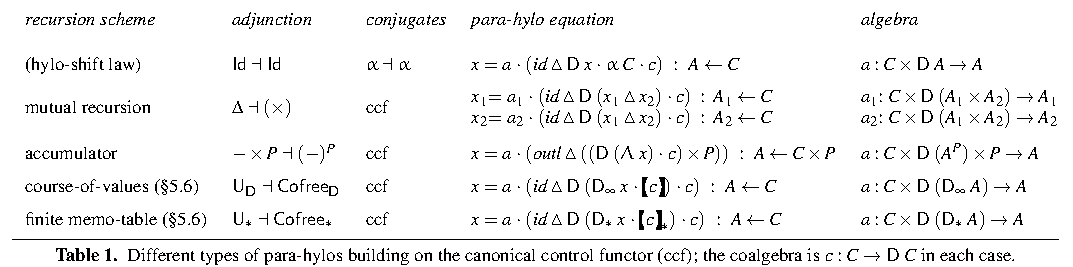
\includegraphics[width=\textwidth]{figures/types-of-parahylos-crop.pdf}\end{sticky}

  \Put(40,290){%
    \begin{onlyenv}<2>
    \begin{minipage}{.86\columnwidth}
    \begin{greenbox}
      \small
      \begin{itemize}
        \item Every complex recursion scheme is a hylomorphism via its associated adjunction/conjugate pair
        \item (e.g) Folds with parameters (accumulators) use the curry/uncurry adjunction
        \item A recursion scheme from comonads (RSFCs, Uustalu, Vene, Pardo, 2001) is an conjugate hylomorphism via the coEilenberg-Moore category for the cofree comonad
      \end{itemize}
    \end{greenbox}
    \end{minipage}
    \end{onlyenv}
  }
\end{frame}

\begin{frame}
  \frametitle{Why Mechanising Hylomorphisms in Coq?}

  \begin{itemize}
    \item Structured Recursion Schemes have been used in Haskell to structure
      functional programs, but they do not ensure termination/productivity
    \item On the other hand, Coq does not capture all recursive definitions
    \item The benefits of formalising hylos in Coq is three fold:
      \begin{itemize}
        \item Giving the Coq programmer a \embf{library} where for most
          recursion schemes they do not have to prove termination properties
        \item \embf{Extracting code} into ML/Haskell to provide termination
          guarantees even in languages with non-termination
        \item Using the laws of hylomorphisms as tactics for \embf{program
          calculation} and \embf{optimisation}
      \end{itemize}
  \end{itemize}
\end{frame}

\begin{frame}
  \frametitle{Challenges}
  \begin{enumerate}
    \item Avoiding axioms: functional extensionality, heterogeneous equality,
      \ldots.
    \item Extracting ``clean'' code: close to what a programmer would have
      written directly in OCaml.
    \item Fixed-points of functors, non-termination, etc.
  \end{enumerate}

  \vspace{.5cm}
  
  \uncover<2->{%
    Our solutions (the remainder of this talk):
    \begin{enumerate}
      \item<2-> Machinery for building setoids, use of decidable predicates, \ldots
      \item<3-> Avoiding type families and indexed types.
      \item<4-> \embf{Containers} \& \embf{recursive coalgebras}
    \end{enumerate}
   }

\end{frame}


\begin{frame}
  \frametitle{Roadmap}
  \centering
  \LARGE

    \begin{sticky}%
      \vspace{-1.5em}
      \begin{tabular}{@{}rl}
        {\textbf{\color{gray}Part I:}} & Extractable Containers in Coq \\
        {\textbf{\color{gray}Part II:}} & Recursive Coalgebras \& Coq Hylomorphisms \\
        {\textbf{\color{gray}Part III:}} & Code Extraction \& Examples 
      \end{tabular}
    \end{sticky}
\end{frame}
% 
% \begin{frame}
%   \frametitle{Why Mechanising Hylomorphisms in Coq?}
% 
%   \begin{itemize}
%   \end{itemize}
% \end{frame}
% 
\begin{frame}
  \vfill
  \centering
  %\begin{beamercolorbox}[sep=8pt,center,shadow=true,rounded=true]{block}
  \begin{sticky}
    \usebeamerfont{title}
    {\normalfont Part I}

    {\normalfont\Large Extractable Containers in Coq}
    \par%
  \end{sticky}
  %\end{beamercolorbox}
  \vfill
\end{frame}

\begin{frame}
  \frametitle{Containers}

  Containers are defined by a  pair $S \triangleleft P$:\blfootnote{%
    Abbott, Altenkirch, Ghani: \textbf{Categories of Containers}. FoSSaCS 2003.
  }
  \begin{itemize}
    \item a type of \alert{shapes} $S : \mathsf{Type}$
    \item a \alert{family} of positions, indexed by shape $P : S \to \mathsf{Type}$
  \end{itemize}

  \vspace{.7cm}
  \uncover<2>{%
    A \alert{container extension} is a functor defined as follows
    \[
      \begin{array}{ll}
        \llbracket S \triangleleft P \rrbracket\; X & = \Sigma_{s : S} P\;s \to X \\[.3cm]
      \llbracket S \triangleleft P \rrbracket\; f & = \lambda (s, p). \; (s, f \circ p)
      \end{array}
    \]
  }
\end{frame}

\begin{frame}
  \frametitle{Example}

  Consider the functor
  \only<1>{$F\; X = \mathcolorbox{white}{1} + \mathcolorbox{white}{X\times X}$}%
  \only<2>{$F\; X = \mathcolorbox{golden}{1} + \mathcolorbox{golden}{X\times X}$}%
  \only<3>{$F\; X = \mathcolorbox{golden}{1} + \mathcolorbox{white}{X\times X}$}%
  \only<4>{$F\; X = \mathcolorbox{white}{1} + \mathcolorbox{golden}{X\times X}$}%
  \vspace{.2cm}

  $S_{F}$ and $P_{F}$ define a container that is isomorphic to $F$

  \[
    \only<1>{S_F = \mathcolorbox{white}{1} + \mathcolorbox{white}{1}}%
    \only<2>{S_F = \mathcolorbox{golden}{1} + \mathcolorbox{golden}{1}}%
    \only<3>{S_F = \mathcolorbox{golden}{1} + \mathcolorbox{white}{1}}%
    \only<4>{S_F = \mathcolorbox{white}{1} + \mathcolorbox{golden}{1}}%
    \tikzmark{shapeC}
    \hspace{.5cm}
      \begin{array}{l}
        \only<1-2,4->{\mathcolorbox{white}{P_{F}\;(\mathsf{inl}\;\sbullet) = 0}}%
        \only<3>{\mathcolorbox{golden}{P_{F}\;(\mathsf{inl}\;\sbullet) = 0}}%
        \tikzmark{pos0}
        \\
        \only<1-3>{\mathcolorbox{white}{P_{F}\;(\mathsf{inr}\;\sbullet) = 1+1}}%
        \only<4>{\mathcolorbox{golden}{P_{F}\;(\mathsf{inr}\;\sbullet) = 1+1}}%
        \tikzmark{pos1}
      \end{array}
   \]
   \vspace{.4cm}

  Examples of objects of types $F\;\mathbb{N}$ (left) and
$\llbracket S_F \triangleleft P_F \rrbracket\;\mathbb{N}$ (right):
   \[\begin{array}{r c l}
        \mathsf{inl}\;\sbullet & \cong & (\mathsf{inl}\;\sbullet, !_{\mathbb{N}})
      \\
        \mathsf{inr}\;(7,9) & \cong &
        (\mathsf{inr}\;\sbullet, \lambda x, \mathsf{case}\;x\;\{%
          \begin{array}{l}
            \mathsf{inl}\;\sbullet \Rightarrow 7;\;\;
            \mathsf{inr}\;\sbullet \Rightarrow 9
          \end{array}
          \})
      \end{array}
  \]

  \begin{overprint}
    \onslide<2>
  \begin{tikzpicture}[overlay,remember picture,shift=(current page.south west)]
    \node[label] at (12,7) (cos)
      {Two cases (``shapes'')};
  \end{tikzpicture}
  \end{overprint}
  \begin{overprint}\onslide<3>
  \begin{tikzpicture}[overlay,remember picture,shift=(current page.south west)]
    \node[label] at (10,8) (copl)
      {No positions on the left shape};
  \end{tikzpicture}
  \end{overprint}
  \begin{overprint}\onslide<4>
  \begin{tikzpicture}[overlay,remember picture,shift=(current page.south west)]
    \node[label] at (10,8) (copl)
      {Two positions on the right shape};
  \end{tikzpicture}
  \end{overprint}
\end{frame}

\begin{frame}[fragile]
  \frametitle{Mechanising Containers: Setoids and Morphisms}
  To avoid the functional extensionality axiom, we use:
  \begin{itemize}
    \item \embf{setoids}: types with an associated equivalence
    \item \embf{proper morphisms} of the respectfulness relation: functions
      that map related inputs to related outputs
  \end{itemize}
  \vspace{.6cm}
  \begin{tabular}{@{}rl@{}}
    \alert{Setoids:} & Given \colorbox{lime}{\coq{setoid A}}, and
  \colorbox{lime}{\coq{x y : A}}, we write 
  \colorbox{lime}{\coq{x =e y : Prop}}.
    \\[.5cm]
    \alert{Morphisms}: & Given 
  \colorbox{lime}{\coq{setoid A}} and 
  \colorbox{lime}{\coq{setoid B}}, we write
  \colorbox{lime}{\coq{f : A ~> B}}.
  \end{tabular}

  \Put(30,160){%
    \begin{onlyenv}<2>
    \begin{minipage}{.86\columnwidth}
    \begin{greenbox}
      \small
      \begin{itemize}
        \item We provide automatic coercion from \coq{A ~> B} to \coq{A -> B}.
        \item Coq's extraction mechanism ignores the \coq{Prop} field.
        \item We provide a (very basic!) mechanism to help building morphisms.
        \item Building on top of setoids \& morphisms allows the  use of Coq's
\alert{generalised rewriting}.
      \end{itemize}
    \end{greenbox}
    \end{minipage}
    \end{onlyenv}
  }
\end{frame}

\begin{frame}[fragile]
  \frametitle{Containers in Coq: A Bad Attempt}
  Assume a \coq{Shape : Type} and \coq{Pos : Shape -> Type}.
  \vspace{.4cm}

  We can define a container extension in the straightforward way:
  \begin{minted}{coq}
Record App (X : Type) :=
  MkCont { shape : Shape; contents : Pos shape -> X }.
  \end{minted}
  \vspace{.2cm}

  \begin{overprint}
    \onslide<2->
  \begin{center}
  \begin{minipage}{.8\columnwidth}
    \begin{infobox}
      \begin{itemize}
        \item The above definition forces us to use dependent equality and
          UIP/Axiom K/\ldots E.g.: dealing with  \coq{eq_dep s1 p1 s2 p2} if
          \coq{p1 : Pos s1} and \coq{p2 : Pos s2}.
        \item Type families lead to OCaml code with \ocaml{Obj.magic}.
      \end{itemize}
    \end{infobox}
  \end{minipage}
  \end{center}
  \end{overprint}
\end{frame}

\begin{frame}[fragile]
  \frametitle{Extractable Containers in Coq (I)}

  Observations:
  \begin{enumerate}
    \item UIP is \alert{not an axiom} in Coq for types with a \alert{decidable
      equality}.
    \item If a type family is defined as a \alert{predicate subtype}, Coq can
      erase the predicate and extract code that is equivalent to the supertype.
      E.g. \coq{{x | P x}} for some \coq{P : X -> Prop}.
  \end{enumerate}
\end{frame}

\begin{frame}[fragile]
  \frametitle{Extractable Containers in Coq (and II)}
  Our containers are defined by:
  \begin{itemize}
    \item \coq{Sh : Type}: type of shapes
    \item \coq{Po : Type}: type of \alert{all} positions
    \item \coq{valid : Sh * Po ~> bool}
      \begin{itemize}
        \item[] \alert{decidable} predicate stating when a pair shape/position is valid
      \end{itemize}
  \end{itemize}
  \vspace{.6cm}

  Container extensions that lead to ``clean'' code extraction:
  \begin{coqcode}
    Record App (X : Type)
    := MkCont { shape : Sh;
                contents : {p | valid (shape, p)} -> X
              }.
  \end{coqcode}
  \Put(40,290){%
    \begin{onlyenv}<2>
    \begin{minipage}{.86\columnwidth}
    \begin{greenbox}
      \small
      \begin{itemize}
        \item All proofs of the form \coq{V1 V2 : valid(s,p) = true} are
              provably equal in Coq to \coq{eq_refl}.
        \item Given \coq{p1 p2 : {p | valid(s, p)}}, \coq{p1 = p2} iff \coq{proj1_sig p1 = proj1_sig p2}.
        \item Extraction will treat the contents of container extensions equivalently to
              \coq{contents : Po -> X}
              \item[] (\ul{no unsafe coercions}).
      \end{itemize}
    \end{greenbox}
    \end{minipage}
    \end{onlyenv}
  }
\end{frame}

\begin{frame}[fragile]
  \frametitle{Example: $F\; X = 1 + X \times X$}

\begin{onlyenv}<1>
  Container definition:
  \vspace{.2cm}

\begin{coqcode}
Inductive ShapeF := Lbranch | Rbranch.
Inductive PosF := Lpos | Rpos.

Definition validF (x : ShapeF * PosF) : bool
  := match fst x with | Lbranch => false | Rbranch => true end.
\end{coqcode}
\end{onlyenv}
\begin{onlyenv}<2>
  Example object equivalent to $\mathsf{inr}\;(7,8)$
  \vspace{.2cm}

\begin{coqcode}
Example e1 : App nat :=
  MkCont Rbranch (fun p => match elem p with
                           | Lpos => 7 | Rpos => 8
                           end).
\end{coqcode}
\end{onlyenv}
\end{frame}

%\begin{frame}
%  \frametitle{Container Equality}
%\end{frame}


\begin{frame}
  The argument of container extensions occurs in \ul{strictly positive} positions:
  \begin{itemize}
    \item[] We can define \ul{least/greatest fixed points of container extensions}.
  \end{itemize}
  \vspace{.5cm}

  We provide a library of polynomial functors as containers, as well as custom
  shapes (e.g. binary trees) that we use in our examples.
  \vspace{.5cm}

  \vspace{.5cm}
  \textbf{Not discussed:}
  \begin{itemize}
    \item Container morphisms and \ul{natural transformations}
    \item Container composition $S \triangleleft P = (S_1 \triangleleft P_1) \circ (S_2 \triangleleft P_2)$
    \item Container equality
  \end{itemize}

\end{frame}

\begin{frame}
  \vfill
  \centering
  %\begin{beamercolorbox}[sep=8pt,center,shadow=true,rounded=true]{block}
  \begin{sticky}
    \usebeamerfont{title}
    {\normalfont Part II}

    {\normalfont\Large Recursive Coalgebras \& Coq Hylomorphisms}
    \par%
  \end{sticky}
  %\end{beamercolorbox}
  \vfill
\end{frame}

\begin{frame}[fragile]
  \frametitle{Algebras \& Container Initial Algebras}

  The least fixed-point of a container extension \coq{App C} is:
  \begin{coqcode}
    Inductive LFix C := Lin { lin_op : App C (LFix C) }.
  \end{coqcode}
  \vspace{.4cm}

  Algebras are of type \coq{Alg C X = App C X ~> X}.
  \vspace{.4cm}

  \textbf{Catamorphisms:}
  \begin{coqcode}
cata : Alg C X ~> LFix C ~> X

cata_univ : forall (a : Alg C X) (f : LFix C ~> X),
  f \o Lin =e a \o fmap f <-> f =e cata a
  \end{coqcode}
\end{frame}

\begin{frame}[fragile]
  \frametitle{Coalgebras \& Container Terminal Coalgebras}

  The \ul{greatest} fixed-point of a container extension \coq{App C} is:
  \begin{coqcode}
    CoInductive GFix C := Gin { gin_op : App C (GFix C) }.
  \end{coqcode}
  \vspace{.4cm}

  Coalgebras are of type \coq{CoAlg C X = X ~> App C X}.
  \vspace{.4cm}

  \textbf{Anamorphisms:}
  \begin{coqcode}
ana : CoAlg C X ~> X ~> GFix C

ana_univ : forall (c : CoAlg C X) (f : X ~> GFix C),
  gin_op \o f =e fmap f \o c <-> f =e ana c
  \end{coqcode}
\end{frame}

\begin{frame}[fragile]
  \frametitle{Recursive Coalgebras (I)}

  We cannot define \coq{hylo} in Coq using arbitrary coalgebras, because they may not exist...

  \uncover<2->{But they exist for \textbf{recursive coalgebras}.%
    \blfootnote{J. Adámek, S. Milius, L.S. Moss:
\textbf{On Well-Founded and Recursive Coalgebras}. FoSSaCS 2020.}
  }
  \vspace{.6cm}

  \uncover<3->{%
    \textbf{Recursive coalgebras}: coalgebras (\coq{c : CoAlg C X}) that terminate in all inputs.
    \begin{itemize}
      \item<3-> i.e. their anamorphisms only produce \ul{finite trees}.
      \item<4-> i.e. they decompose inputs into ``smaller'' values of type \coq{X}
    \end{itemize}
  }
\end{frame}

\begin{frame}
  \frametitle{Recursive Coalgebras (and II)}

  We define a predicate \coq{RecF c x} that states that \coq{c : CoAlg C X}
terminates on \coq{x : X}.
     \vspace{.4cm}

  Using \coq{RecF}, we define:
    \begin{enumerate}
      \item Recursive coalgebras:

            \coq{RCoAlg C X = {c | forall x, RecF c x}}

      \item Given a well-founded relation \coq{R}, well-founded coalgebras

            \coq{WfCoalg C X = {c | forall x p, R (contents (c x) p) x}}
     \end{enumerate}
     \vspace{.4cm}

    \begin{itemize}
    \item<2-> Definitions (1) and (2) are equivalent
    \item<3-> Our mechanisation represents (2) in terms of (1)
    \item<4-> Termination proofs may be easier using (1) or (2), depending on the
use case
    \end{itemize}
\end{frame}

\begin{frame}[fragile]
  \frametitle{Recursive Hylomorphisms}

  \textbf{Recall:}
\vspace{.2cm}

  Hylomorphisms are solutions to the equation
$f = a \circ \mathsf{fmap}\;f \circ c$.

\vspace{.2cm}
  Due to termination, this solution \ul{may not exist}, or \ul{may not be unique}.

\vspace{.2cm}
  If $c$ is recursive, then the solution \textbf{is unique, and guaranteed to exist}.
\vspace{.4cm}

  \begin{overprint}
    \onslide<2->
    \begin{minipage}{\textwidth}
      \begin{bluebox}
      \begin{coqcode}
Definition hylo_def (a : Alg F B) (c : Coalg F A)
  : forall (x : A), RecF c x -> B :=
  fix f x H :=
    match c x as cx
          return (forall e : Pos (shape cx), RecF c (cont cx e)) -> B
    with
    | MkCont sx cx => fun H => a (MkCont sx (fun e => f (cx e) (H e)))
    end (RecF_inv H).
      \end{coqcode}
      \end{bluebox}
    \end{minipage}
  \end{overprint}

\end{frame}

\begin{frame}[fragile]
  \frametitle{Universal Property of Recursive Hylomorphisms}

  We define wrappers over \coq{hylo_def}:
  \vspace{.2cm}

  \begin{center}
  \begin{minipage}{.6\textwidth}
  \begin{bluebox}
  \begin{coqcode}
hylo : Alg C B ~> RCoAlg C A ~> A ~> B
  \end{coqcode}
  \end{bluebox}
  \end{minipage}
  \end{center}

  \vspace{.6cm}
  From this definition, we can prove the universal property of hylomorphisms.

  Given \coq{a : Alg C B} and \coq{c : RCoAlg C A}:
  \vspace{.2cm}

  \begin{center}
  \begin{minipage}{.6\textwidth}
  \begin{bluebox}
  \begin{coqcode}
hylo_univ : forall f : A ~> B,
  f =e a \o fmap f \o c <-> f = hylo a c
  \end{coqcode}
  \end{bluebox}
  \end{minipage}
  \end{center}

\end{frame}

\begin{frame}[fragile]
  \frametitle{A Note on Recursive Anamorphisms}

  For simplicity, we define \ul{recursive anamorphisms} as
  \coq{rana c = hylo Lin c}.
  \begin{itemize}
  \item This way we avoid the need to convert \coq{GFix} to \coq{LFix}.
  \item We prove (straightforward) that \coq{rana c} is equal to \coq{ana c},
followed by converting the result to \coq{LFix}.
  \end{itemize}

\end{frame}

\begin{frame}[t,fragile]
  \frametitle{Proving the Laws of Hylomorphisms}

The following \coq{hylo_fusion} laws \ul{are straightforward consequences} of
\coq{hylo_univ}.\only<2>{%
  \blfootnote{\tiny{}R. Hinze, N. Wu, J. Gibbons: \textbf{Conjugate
  Hylomorphisms - Or: The Mother of All Structured Recursion Schemes}. POPL
  2015.}
  }
\vspace{.2cm}

  \begin{center}
  \begin{minipage}{.82\textwidth}
  \begin{bluebox}
  \begin{coqcode}
Lemma hylo_fusion_l
    : h \o a =e b \o fmap h -> h \o hylo a c =e hylo b c.

Lemma hylo_fusion_r
    : c \o h =e fmap h \o d -> hylo a c \o h =e hylo a d.

Lemma deforest : cata a \o rana c =e hylo a c.
  \end{coqcode}
  \end{bluebox}
  \end{minipage}
  \end{center}


  \Put(40,90){%
    \begin{onlyenv}<2>
    \begin{minipage}{.86\columnwidth}
      \small
    \begin{greenbox}
      The \ul{proofs in Coq are almost direct copies from pen-and-paper proofs}:
By \coq{hylo_univ}, \coq{hylo b c} is the only arrow making the outer square
commute.
\[\begin{tikzcd}[ampersand replacement=\&, nodes={column sep=5.5em}]
	{t b} \& { ta} \& {tc} \\
	{f\; tb} \& {f\;ta} \& {f\;tc}
	\arrow["h"', from=1-2, to=1-1]
	\arrow["\mathsf{hylo}\;a\;c"', from=1-3, to=1-2]
	\arrow["c", from=1-3, to=2-3]
	\arrow["b", from=2-1, to=1-1]
	\arrow["a", from=2-2, to=1-2]
	\arrow["{\mathsf{fmap}\;h}", from=2-2, to=2-1]
	\arrow["{\mathsf{fmap}\;(\mathsf{hylo}\;a\;c)}", from=2-3, to=2-2]
\end{tikzcd}\]
    \end{greenbox}
    \end{minipage}
    \end{onlyenv}
  }

\end{frame}

\begin{frame}[fragile]
  \begin{center}
    \begin{itemize}
    \item Our formalisation allows to do equational reasoning that closely
mirrors pen-and-paper proofs.
    \item \coq{hylo_fusion} can be applied to \emph{calculate} optimised
programs by fusing simpler specifications in Coq.
    \item This leads to more modular development and proofs, without affecting
the performance of the extracted code.
    \end{itemize}
  \end{center}
\end{frame}

\begin{frame}
  \vfill
  \centering
  %\begin{beamercolorbox}[sep=8pt,center,shadow=true,rounded=true]{block}
  \begin{sticky}
    \usebeamerfont{title}
    {\normalfont Part III}

    {\normalfont\Large Code Extraction \& Examples}
    \par%
  \end{sticky}
  %\end{beamercolorbox}
  \vfill
\end{frame}

\begin{frame}[fragile]
  \frametitle{A Tree Container for Divide \&Conquer}

  Our divide-and-conquer examples use a tree container \coq{TreeC A B} that is
isomorphic to:
  \[
    T\; A\; B\; X = A + B \times X \times X
  \]
  \vspace{.3cm}

  Given two setoids \coq{A} and \coq{B}, we define the following wrappers in
Coq:
\vspace{.4cm}

\begin{center}
\begin{minipage}{.65\textwidth}
\begin{bluebox}
  \begin{coqcode}
a_node : B ~> X ~> X ~> App (TreeC A B) X
a_leaf : A ~> App (TreeC A B) X
a_out : App (TreeC A B) X ~> A + B * X * X
  \end{coqcode}
\end{bluebox}
\end{minipage}
\end{center}
\end{frame}

\begin{frame}[fragile]
  \frametitle{Quicksort Definition}

  \begin{coqcode}
Definition mergeF (x : App (TreeC unit int) (list int)) : list int :=
  match a_out x with
  | inl _ => nil
  | inr (p, l, r) => List.app l (h :: r)
  end.

Definition splitF (l : list int) : App (TreeC unit int) (list int) :=
  match x with
  | nil => a_leaf tt
  | cons h t => let (l, r) := List.partition (fun x => x <=? h) t in
                a_node h l r
  end.
  \end{coqcode}
\end{frame}

\begin{frame}[fragile]
  \frametitle{Quicksort Extraction}
    \begin{minipage}{.86\columnwidth}
    \begin{bluebox}
    \begin{coqcode}
Definition qsort := hylo merge split.
Extraction qsort.
    \end{coqcode}
    \end{bluebox}
    \end{minipage}

  \vspace{.6cm}

    \begin{overprint}
    \onslide<2->
    \begin{minipage}{.86\columnwidth}
    \begin{greenbox}
    \begin{ocamlcode}
let rec qsort = function
| [] -> []
| h :: t ->
  let (l, r) = partition (fun x0 -> leb x0 h) t in
  let x0 = fun e -> qsort (match e with
                           | Lbranch -> l
                           | Rbranch -> r) in
  app (x0 Lbranch) (h :: (x0 Rbranch))
    \end{ocamlcode}
    \end{greenbox}
    \end{minipage}
    \end{overprint}
\end{frame}

\begin{frame}[fragile]
  \frametitle{Using Hylo-fusion for Program Optimisation}

  \begin{onlyenv}<1>
    \begin{minipage}{.86\columnwidth}
    \begin{bluebox}
    \begin{coqcode}
Definition qsort_times_two
  : {f | f =e map times_two \o hylo merge split}.
  eapply exist.
  (* ... *)
  rewrite (hylo_fusion_l H); reflexivity.
Defined.

Extraction qsort_times_two.
    \end{coqcode}
    \end{bluebox}
    \end{minipage}
  \end{onlyenv}

  \begin{onlyenv}<2>
    \begin{minipage}{.92\columnwidth}
    \begin{greenbox}
    \begin{ocamlcode}
let rec qsort_times_two = function
| [] -> []
| h :: t ->
  let (l, r) = partition (fun x0 -> leb x0 h) t in
  let x0 = fun p -> qsort_times_two (match p with
                                     | Lbranch -> l
                                     | Rbranch -> r) in
  app (x0 Lbranch) ((mul (Uint63.of_int (2)) h) :: (x0 Rbranch))
    \end{ocamlcode}
    \end{greenbox}
    \end{minipage}
    \end{onlyenv}
\end{frame}

\begin{frame}
  \frametitle{A Recursion Scheme for Dynamic Programming}
  Given a functor $G$, we can construct a
  memoisation table $G_{\ast} A = \mu X. A \times G X$.

  We can index the memoisation table, extract its head, and insert a new element:
  \[
    \begin{array}{@{}l@{}}
      \mathsf{look} : \mathbb{N} \times G_{{\ast}}A \to 1 + A \hspace{.5cm}
      \mathsf{head} : G_{\ast} A \to A \hspace{.5cm}
      \mathsf{Cons} : A \times G (G_{\ast} A) \to G_{\ast} A
    \end{array}
  \]

  \vspace{.2cm}
  Given an algebra $a : G(G_{\ast}A)\to A$, we can construct
  \[ a'= \mathsf{Cons} \circ \mathsf{pair}\; a\; \mathsf{id} : G(G_{\ast} A) \to G_{\ast} A
  \]
  $a'$ computes the current value, as well as storing it
  in the memoisation table.
  \vspace{.3cm}

    \begin{overprint}
    \onslide<2->
    \begin{center}
    \begin{minipage}{.7\columnwidth}
    \begin{greenbox}
      \textbf{Dynamorphisms:} \hspace{.3cm}
      $\mathsf{dyna}\; a\;c = \mathsf{head}\circ \mathsf{hylo}\;a'\;c$
    \end{greenbox}
    \end{minipage}
    \end{center}
    \end{overprint}

\end{frame}

\begin{frame}[fragile]
  \frametitle{Knapsack}
  \begin{onlyenv}<1>
  \begin{bluebox}
  \begin{center}
  \begin{coqcode}
Definition knapsack_alg (wvs : list (nat * int))
  (x : App NatF (Table NatF int)) : int
  := match x with
     | MkCont sx kx =>
       match sx with
       | inl tt => fun _ => 0
       | inr tt => fun kx => let table := kx posR in
                             max_int 0 (memo_knap table wvs)
       end kx
     end.
  \end{coqcode}
  \end{center}
  \end{bluebox}
  \end{onlyenv}
  \begin{onlyenv}<2>
  \begin{greenbox}
  \begin{center}
  \begin{ocamlcode}
let knapsack wvs x =
  ((let rec f n =
    if n=0 then
      { lFix_out = { shape = Uint63.of_int 0;
                     cont  = fun _ -> f 0 } }
    else
      let fn = f (n-1) in
      { lFix_out = { shape = max_int (Uint63.of_int 0)
                                     (memo_knapsack fn wvs);
                     cont = fun e -> fn } }
  ) in f x).lFix_out.shape
  \end{ocamlcode}
  \end{center}
  \end{greenbox}
  \end{onlyenv}
\end{frame}

\begin{frame}
  \vfill
  \centering
  %\begin{beamercolorbox}[sep=8pt,center,shadow=true,rounded=true]{block}
  \begin{sticky}
    \usebeamerfont{title}
    {\normalfont Wrap-up}

    {\normalfont\Large \phantom{wrap-up}}
    \par%
  \end{sticky}
  %\end{beamercolorbox}
  \vfill
\end{frame}

\begin{frame}
  \frametitle{Summary}

  \textbf{Hylomorphisms in Coq}
  \begin{itemize}
  \item Modular specification of functions, without sacrificing performance
thanks to \coq{hylo_fusion}.
  \item Modular treatment of divide-and-conquer and termination proofs using recursive coalgebras.
  \item Clean OCaml code extraction.
  \end{itemize}

  \vspace{.6cm}
  \begin{overprint}
    \onslide<2>
  \textbf{Future work}:
  \begin{itemize}
    \item Improve extraction \& inlining.
    \item Effects.
    \item Dealing with setoids \& equalities.
  \end{itemize}
  \end{overprint}

\end{frame}

\end{document}
